% !TeX root = thesis.tex
%

\chapter{Exploratory Data Analysis Plots} \label{ap1:eda_plots}

This appendix complements the exploratory data analysis presented in
Section~\ref{sec:eda}. The main text discusses only the variables and phenomena that
directly motivated a subsequent methodological decision. This appendix reports the
remaining material in full, so that the behaviour of every continuous process variable
can be inspected without cluttering the main narrative.

Sections~\ref{ap1:timeseries} and~\ref{ap1:distributions} cover the full collection
period, prior to any filtering by operating mode or partitioning into sessions, and
therefore correspond to the same 39{,}175 observations used for
Table~\ref{tab:eda_summary}. Section~\ref{ap1:correlation} reports the numerical values
behind the correlation matrix shown in Figure~\ref{fig:eda_correlation}, and
Section~\ref{ap1:sessions} presents the eleven production sessions retained after data
cleaning individually.

\section{Time Series Over the Full Collection Period} \label{ap1:timeseries}

Figures~\ref{fig:ap1_ts_pressure} to~\ref{fig:ap1_ts_vsd} show every continuous process
variable over the entire collection period, grouped by measurement type. The variables
are plotted as recorded, without any filtering by operating mode, so that the periods
during which the plant was not in production remain visible: these appear as the
intervals where the pump's electrical and mechanical variables drop to zero, and are the
same intervals removed during data cleaning.

\begin{figure}[htbp]
    \centering
    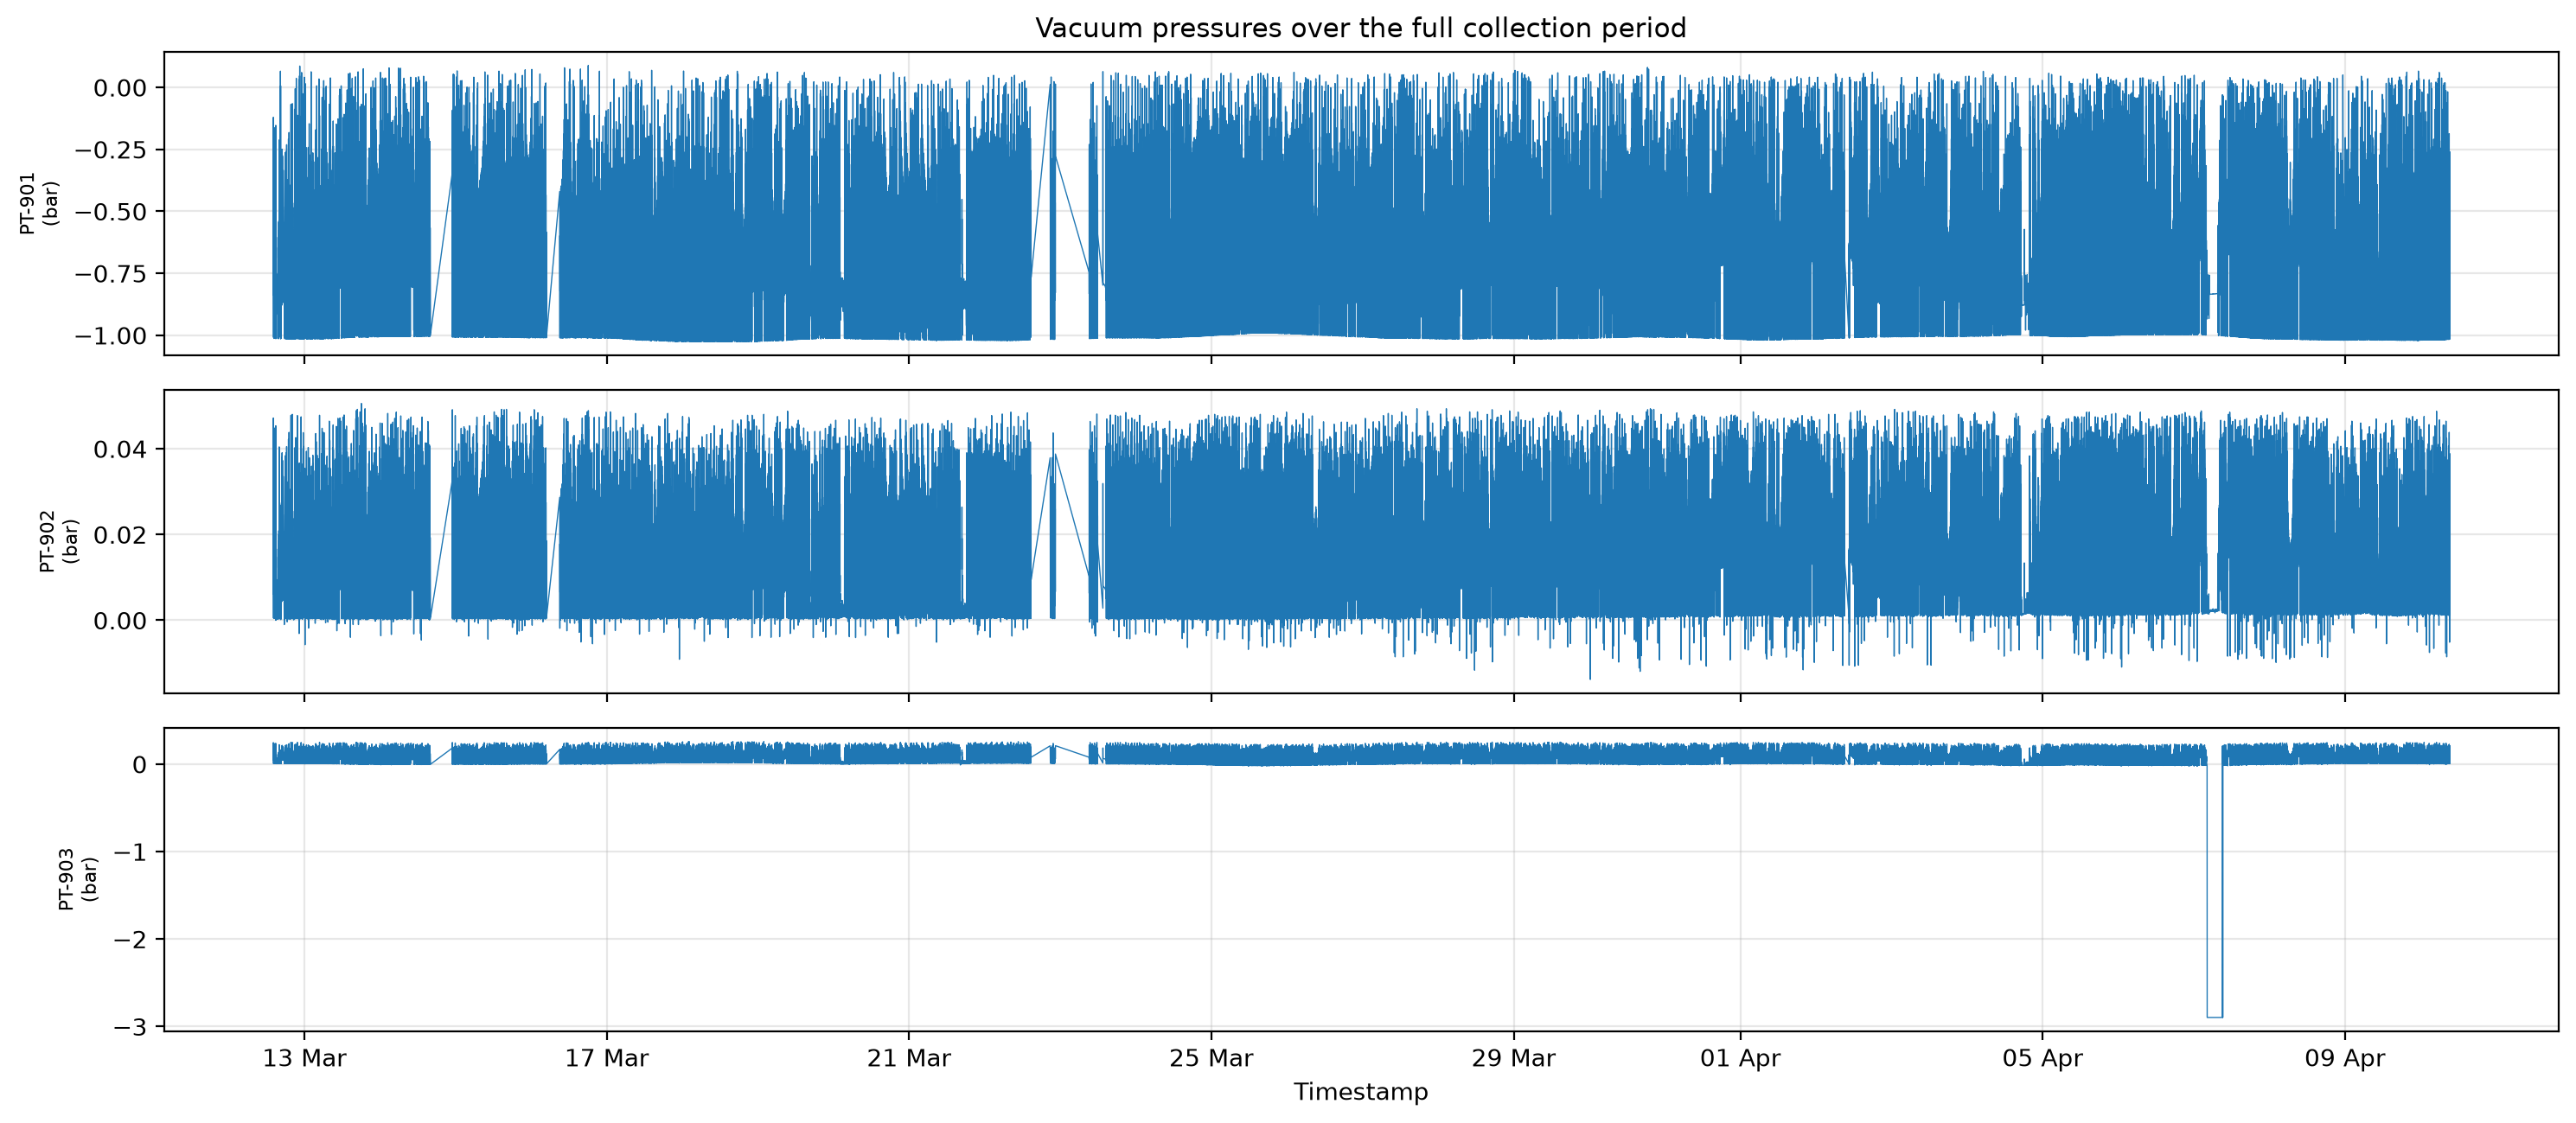
\includegraphics[width=0.95\textwidth]{imgs/eda_appendix_timeseries_pressure.png}
    \caption{Vacuum pressure variables (PT-901, PT-902, PT-903) over the full collection
    period.}
    \label{fig:ap1_ts_pressure}
\end{figure}

\begin{figure}[htbp]
    \centering
    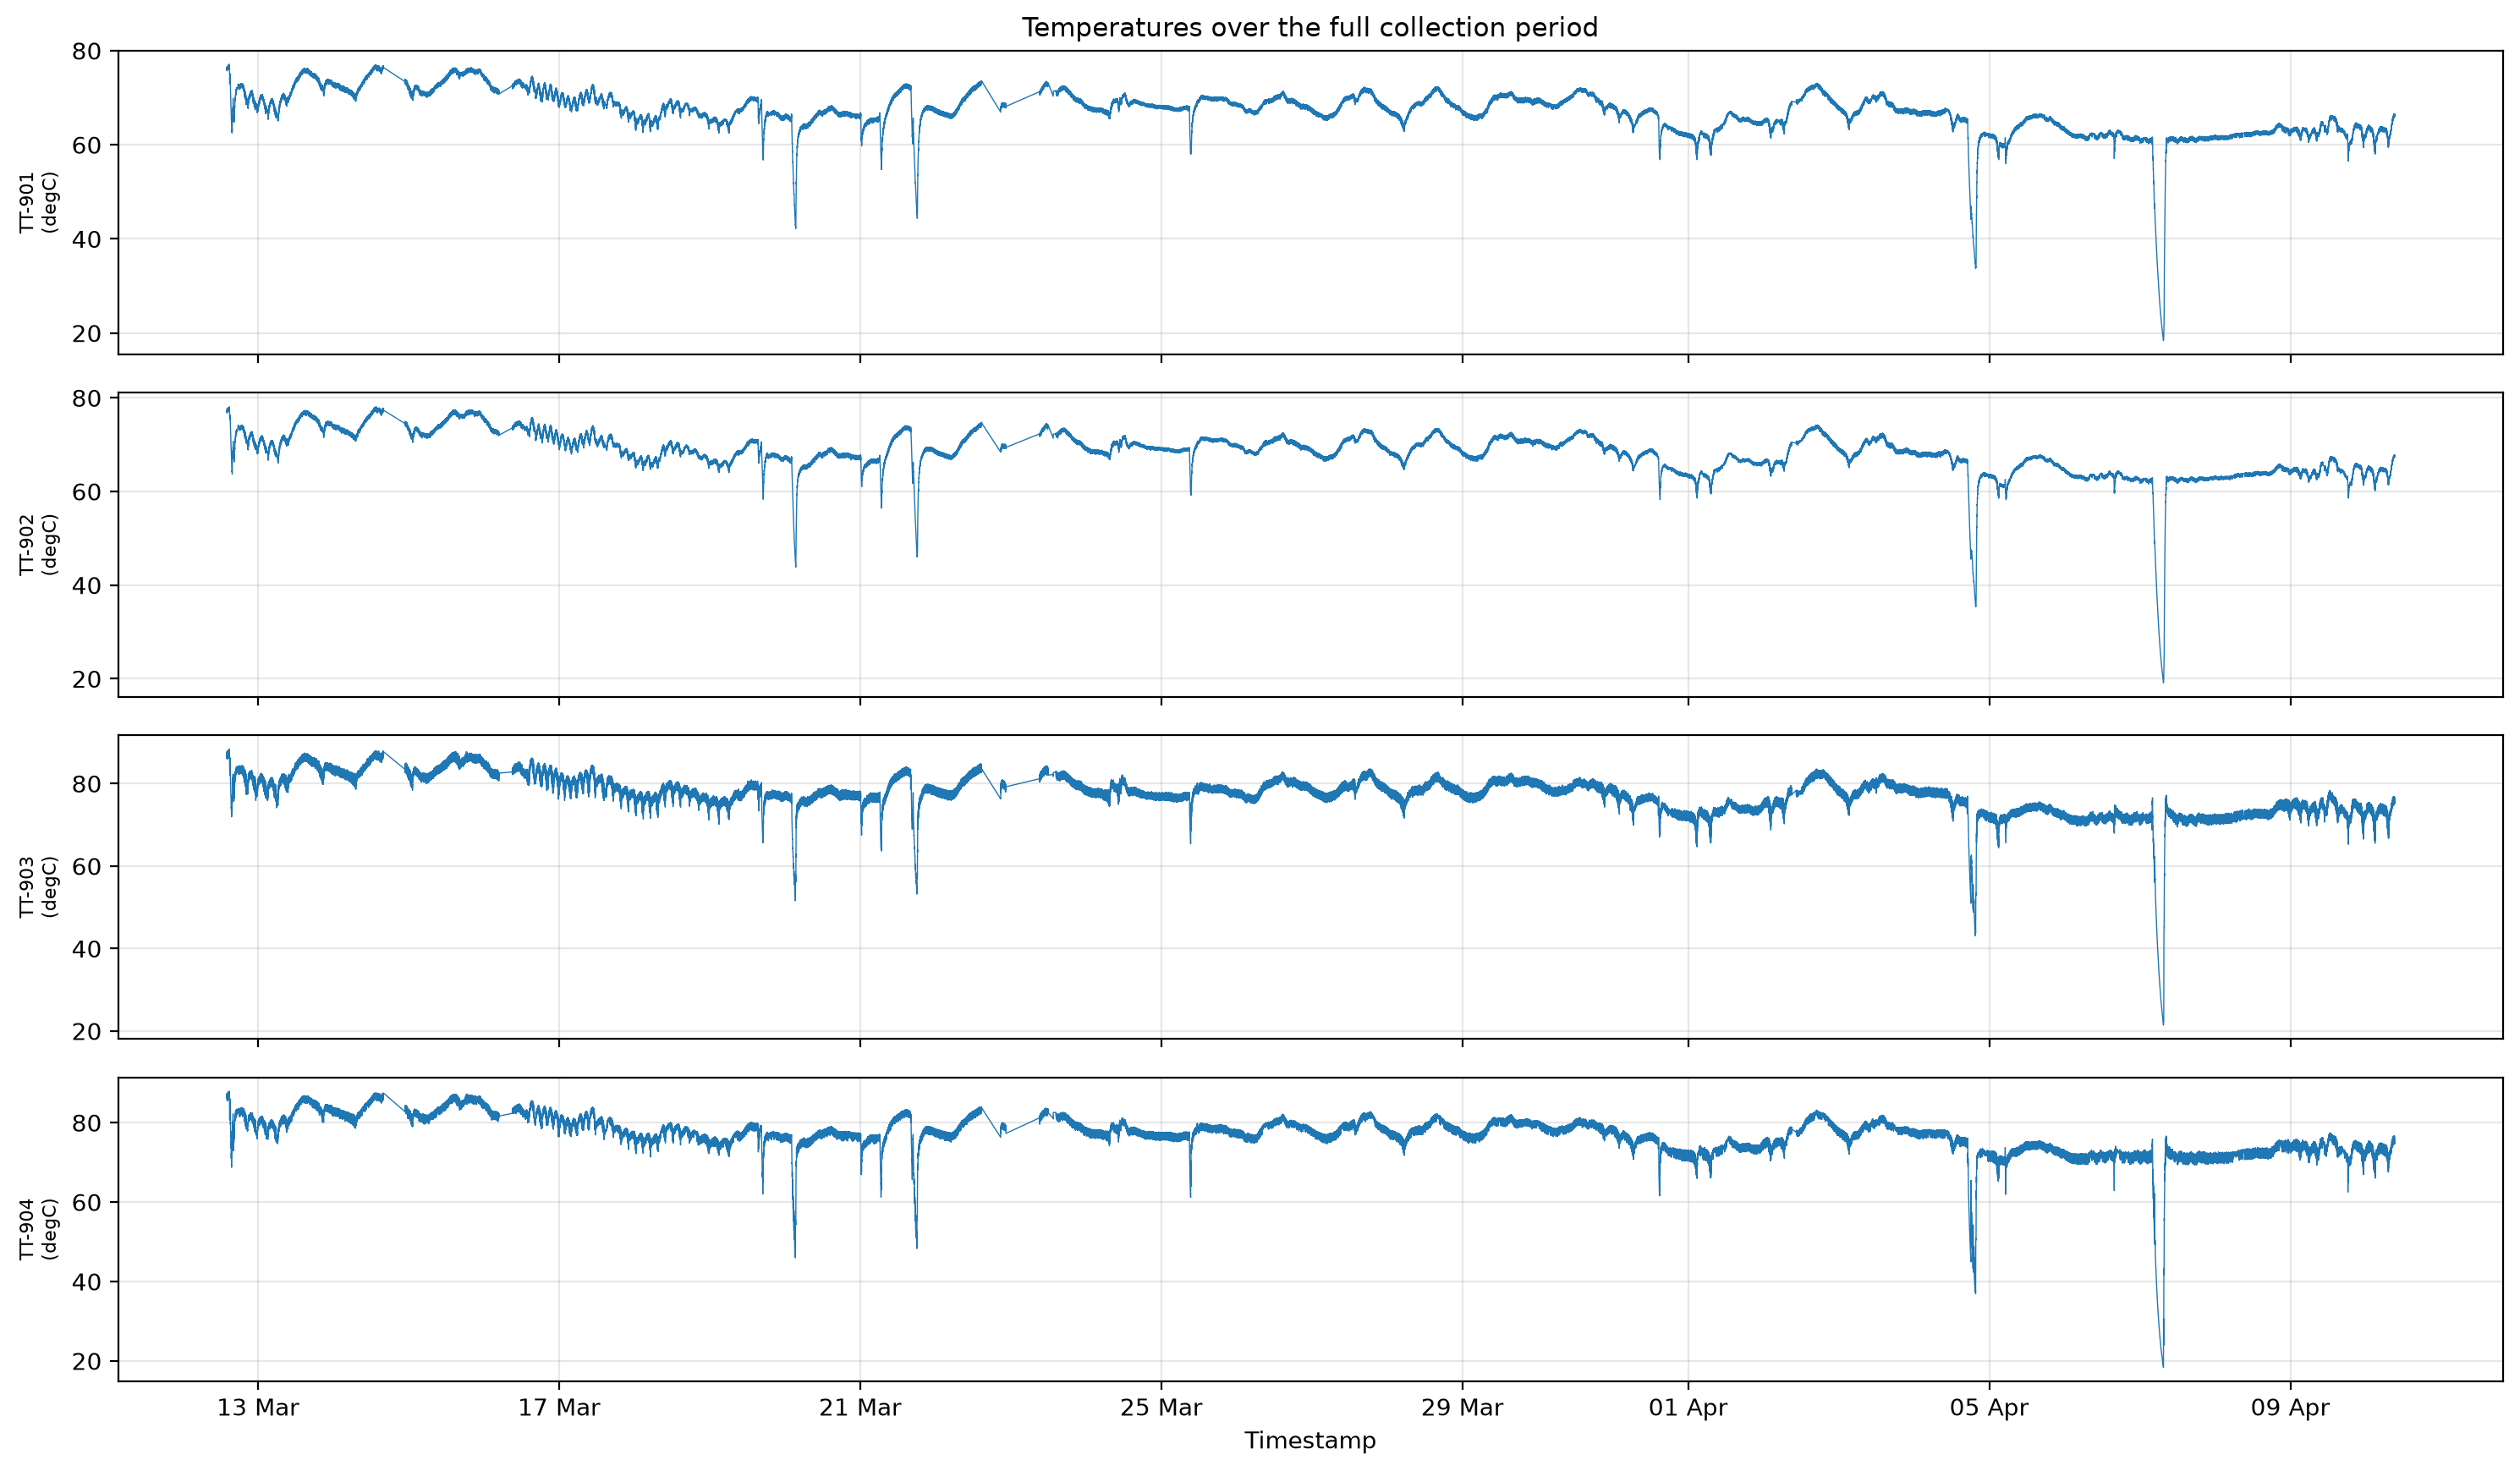
\includegraphics[width=0.95\textwidth]{imgs/eda_appendix_timeseries_temperature.png}
    \caption{Temperature variables (TT-901 to TT-904) over the full collection period.}
    \label{fig:ap1_ts_temperature}
\end{figure}

\begin{figure}[htbp]
    \centering
    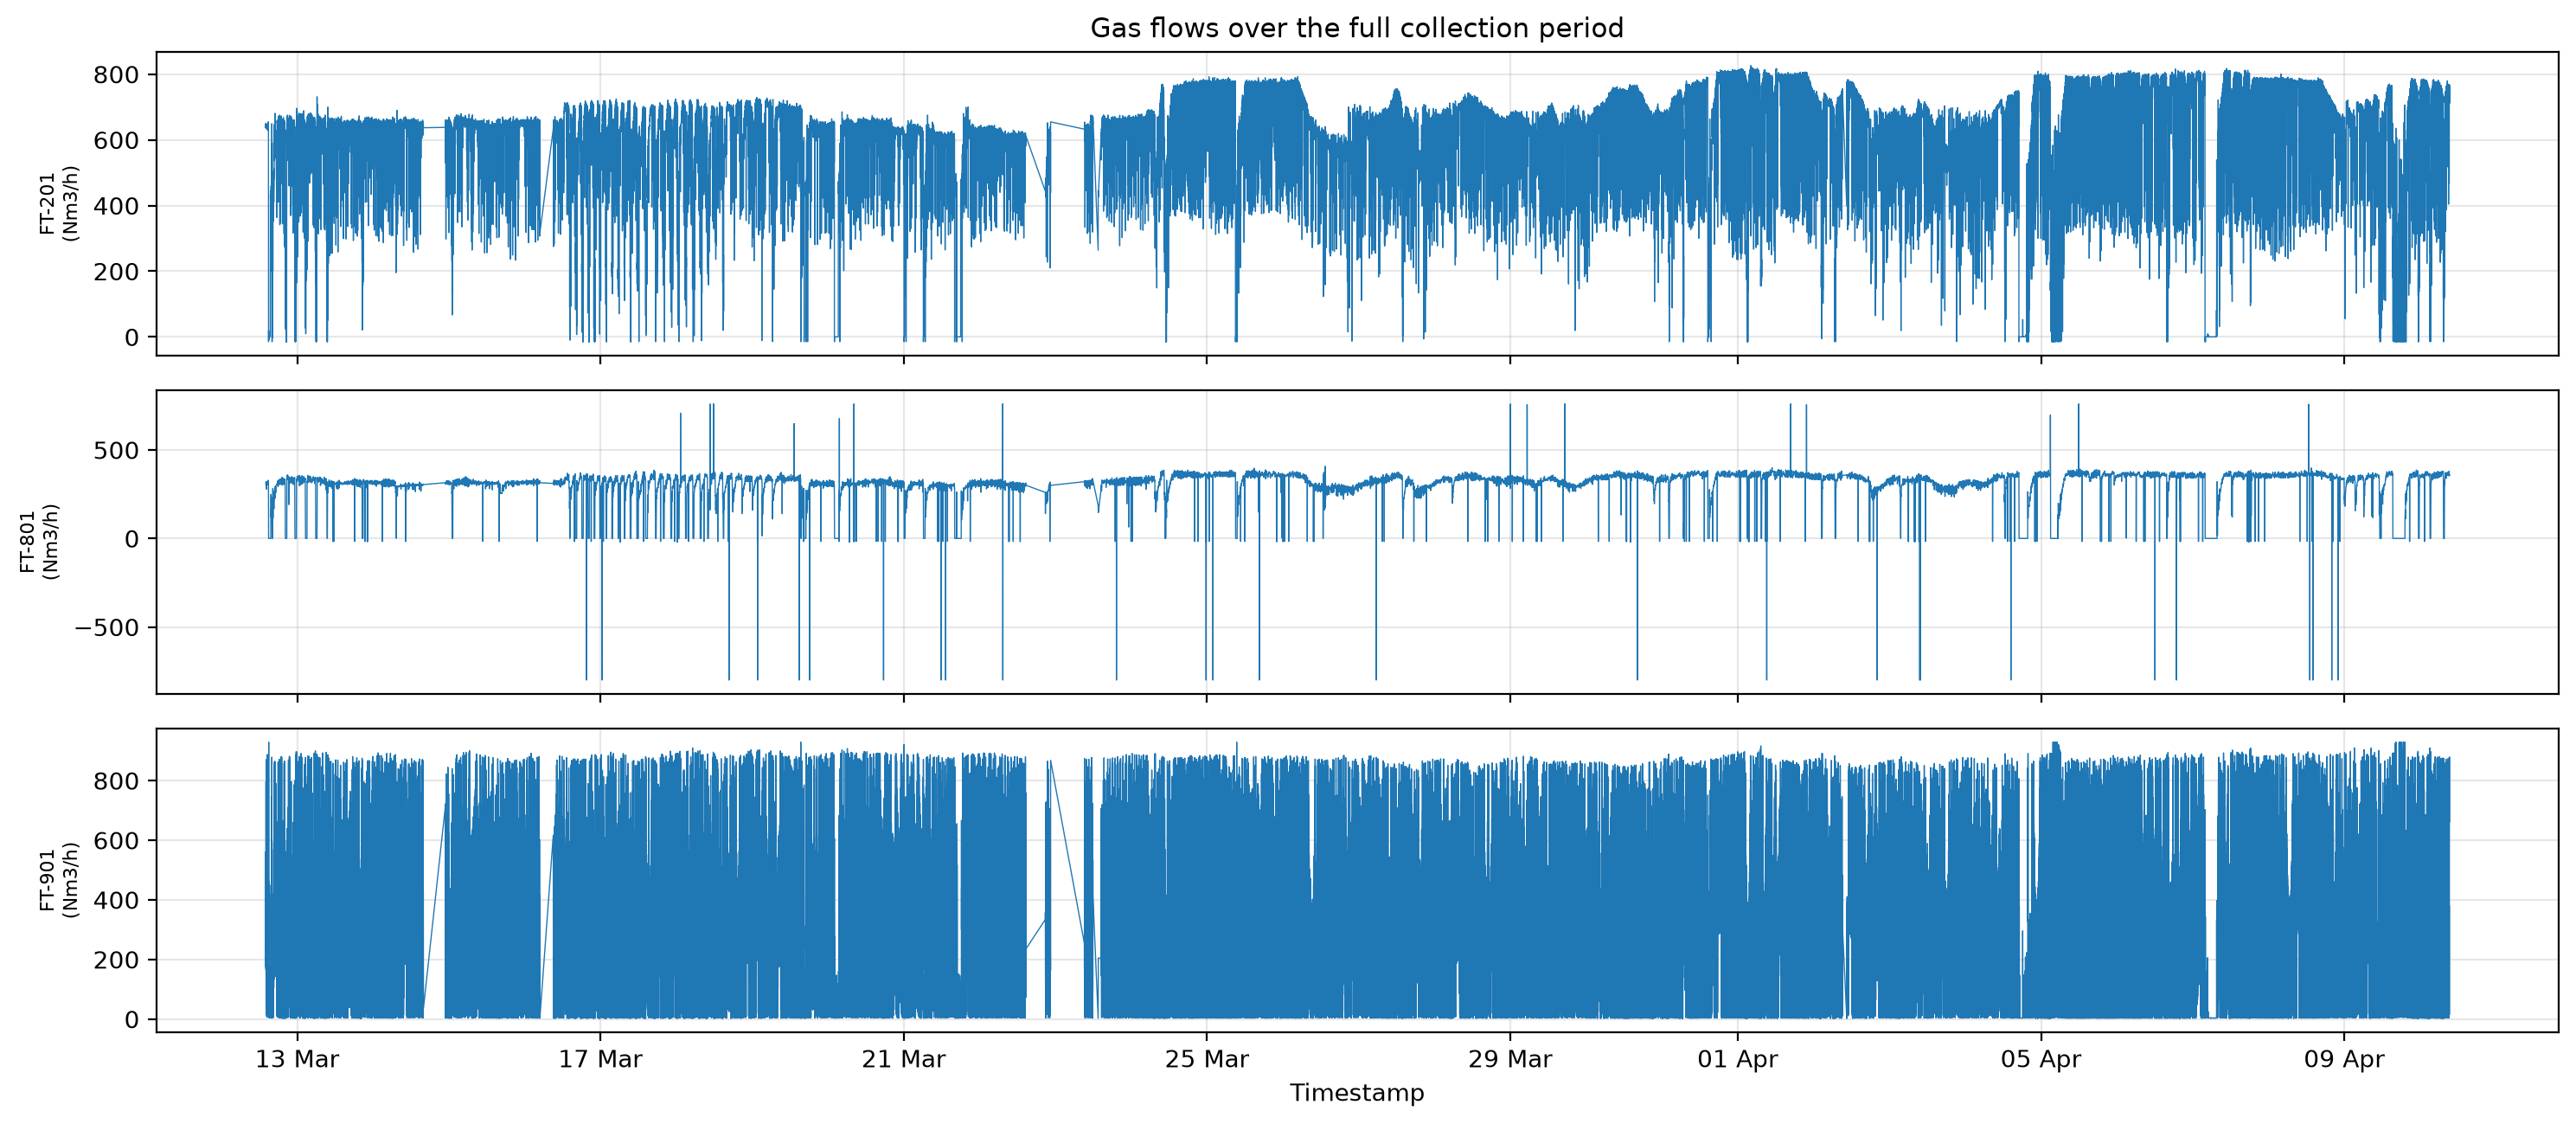
\includegraphics[width=0.95\textwidth]{imgs/eda_appendix_timeseries_flow.png}
    \caption{Gas flow variables (FT-201, FT-801, FT-901) over the full collection period.}
    \label{fig:ap1_ts_flow}
\end{figure}

\begin{figure}[htbp]
    \centering
    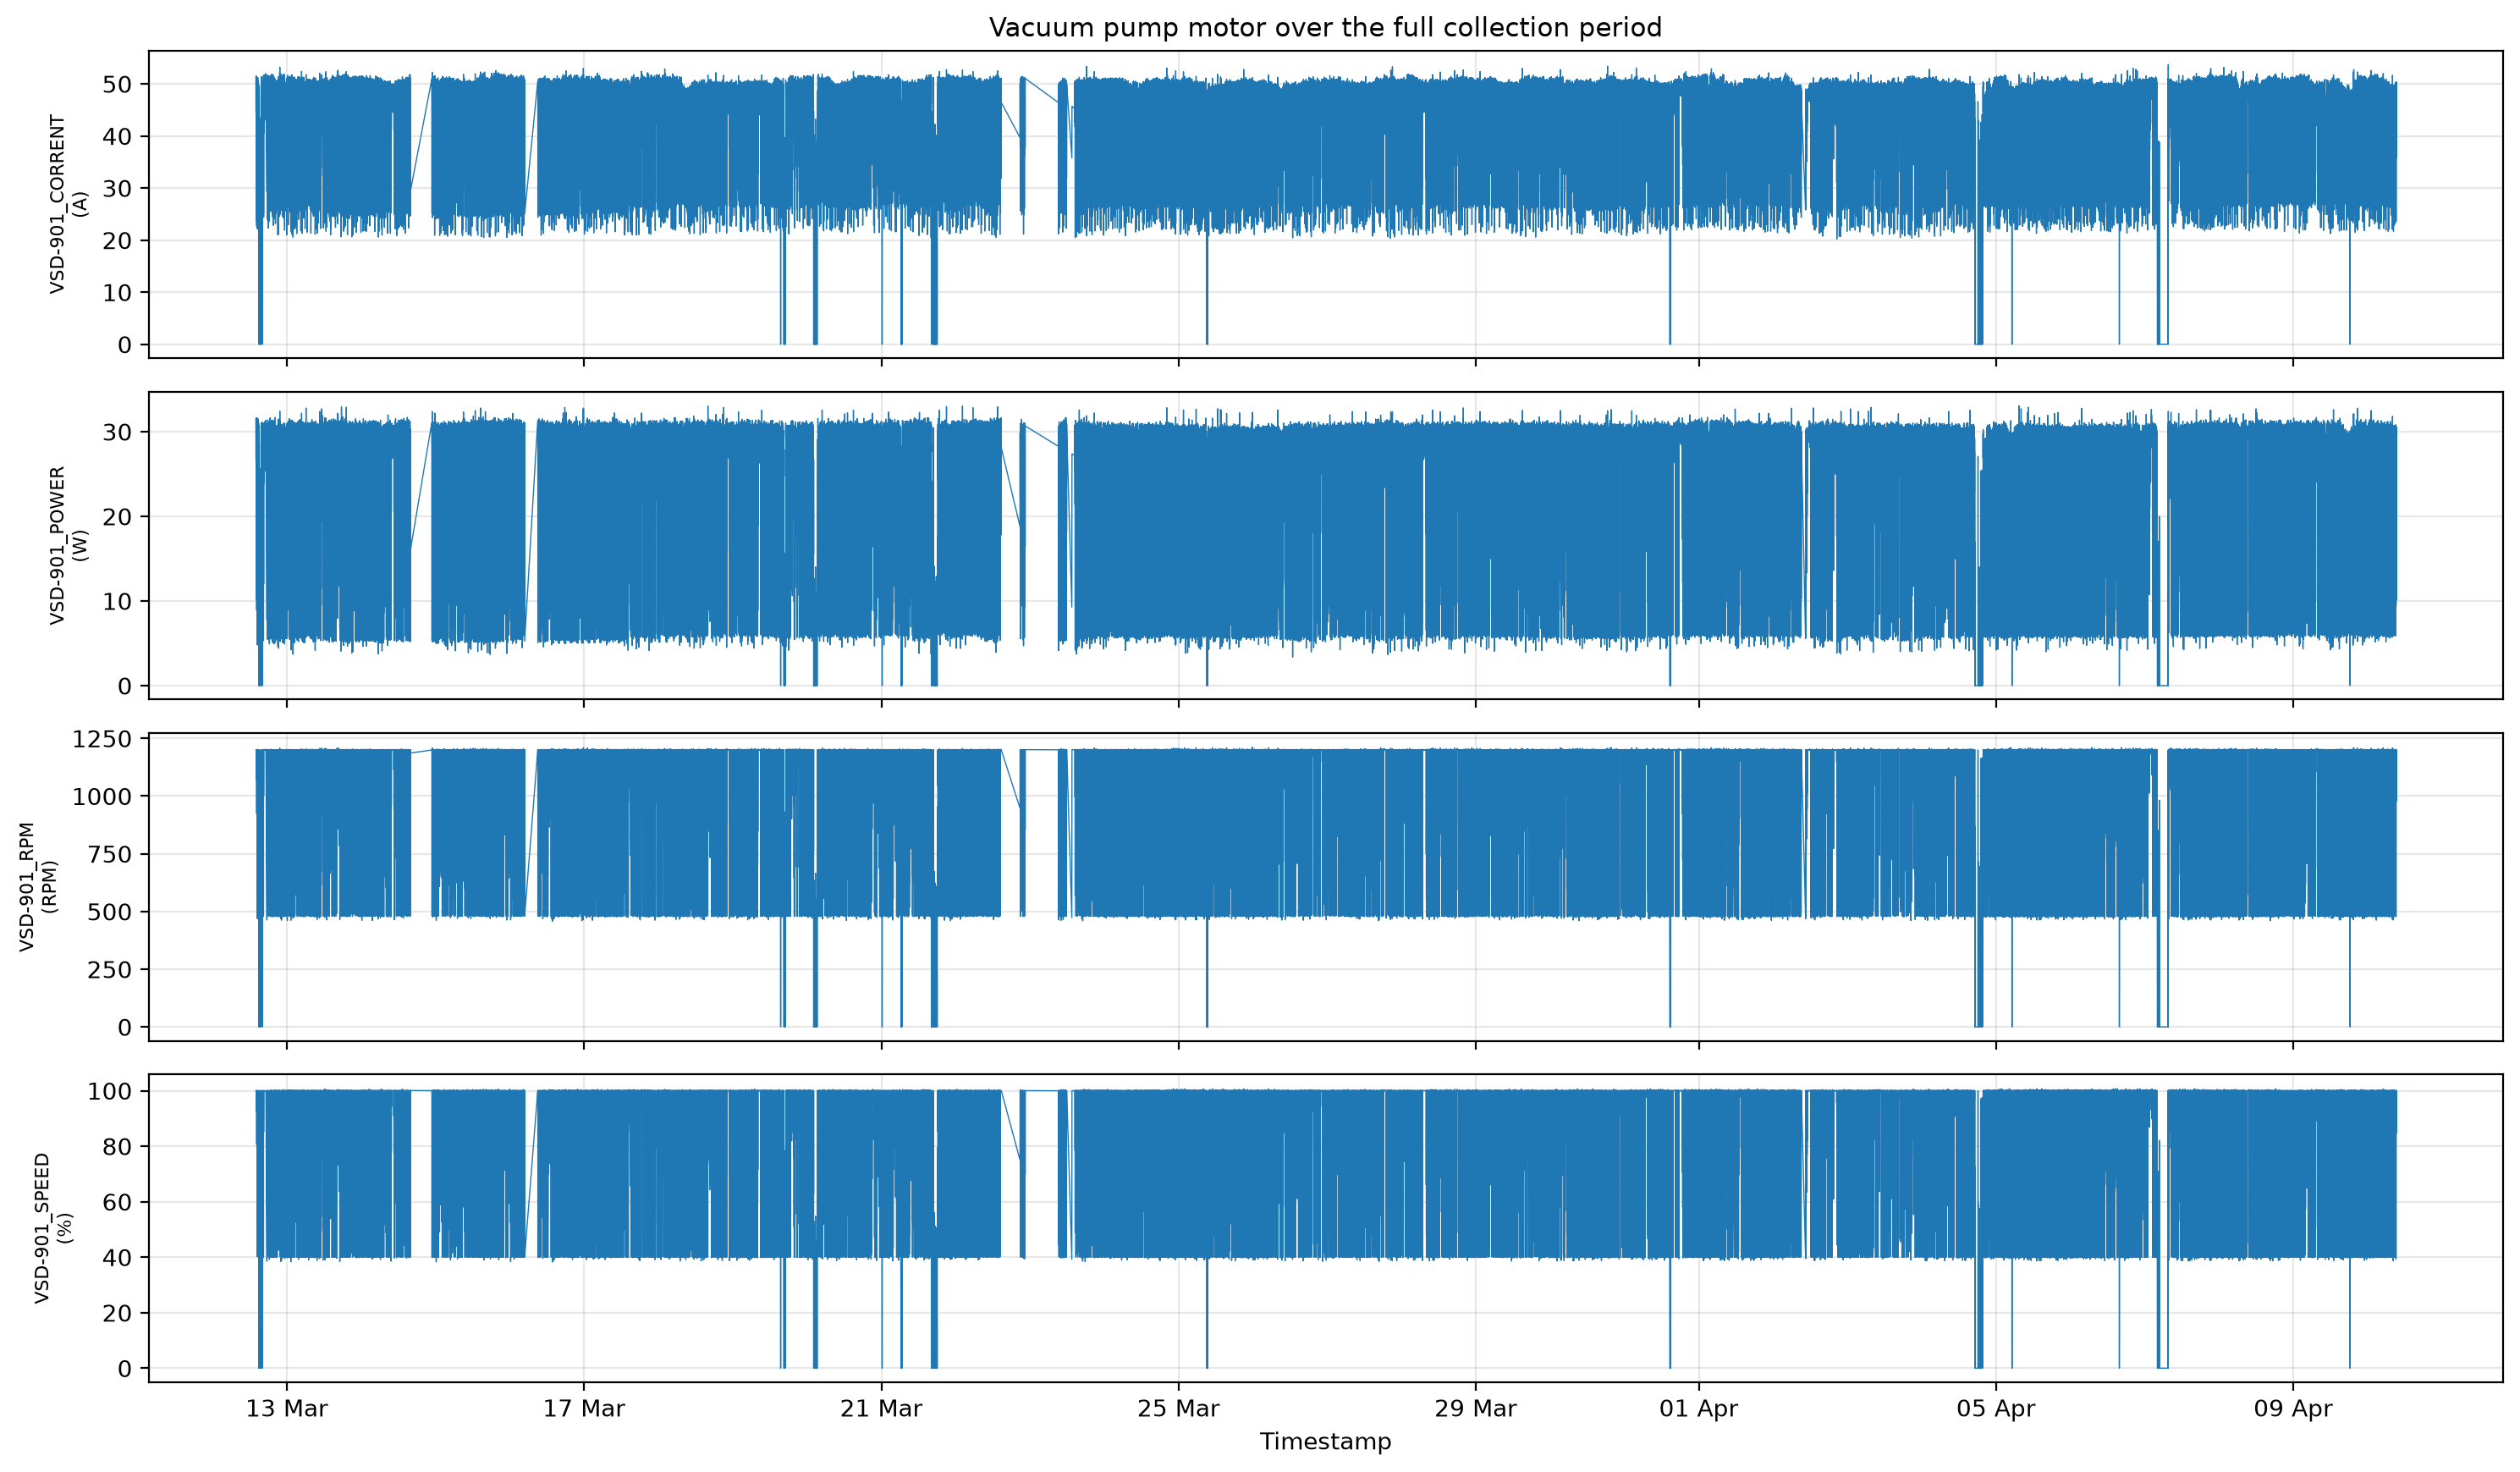
\includegraphics[width=0.95\textwidth]{imgs/eda_appendix_timeseries_vsd.png}
    \caption{Vacuum pump motor variables (VSD-901\_CORRENT, VSD-901\_POWER,
    VSD-901\_RPM, VSD-901\_SPEED) over the full collection period.}
    \label{fig:ap1_ts_vsd}
\end{figure}

\section{Distributions of the Continuous Process Variables} \label{ap1:distributions}

Figure~\ref{fig:ap1_distributions} presents the distribution of each of the fourteen
continuous process variables over the full collection period. Two adjustments were made
so that the shape of the bulk of each distribution remains legible: the frozen PT-903
readings at $-2.896296$~bar and the isolated FT-801 readings at $-800.000000$, both
discussed in Section~\ref{sec:eda}, are excluded from their respective histograms, since
a handful of observations several orders of magnitude away from the rest would otherwise
compress the entire distribution into a single bin.

The bimodal shape visible in the pump's electrical and mechanical variables reflects the
two operating regimes present in the unfiltered data, with the mode near zero
corresponding to the periods during which the plant was not in production.

\begin{figure}[htbp]
    \centering
    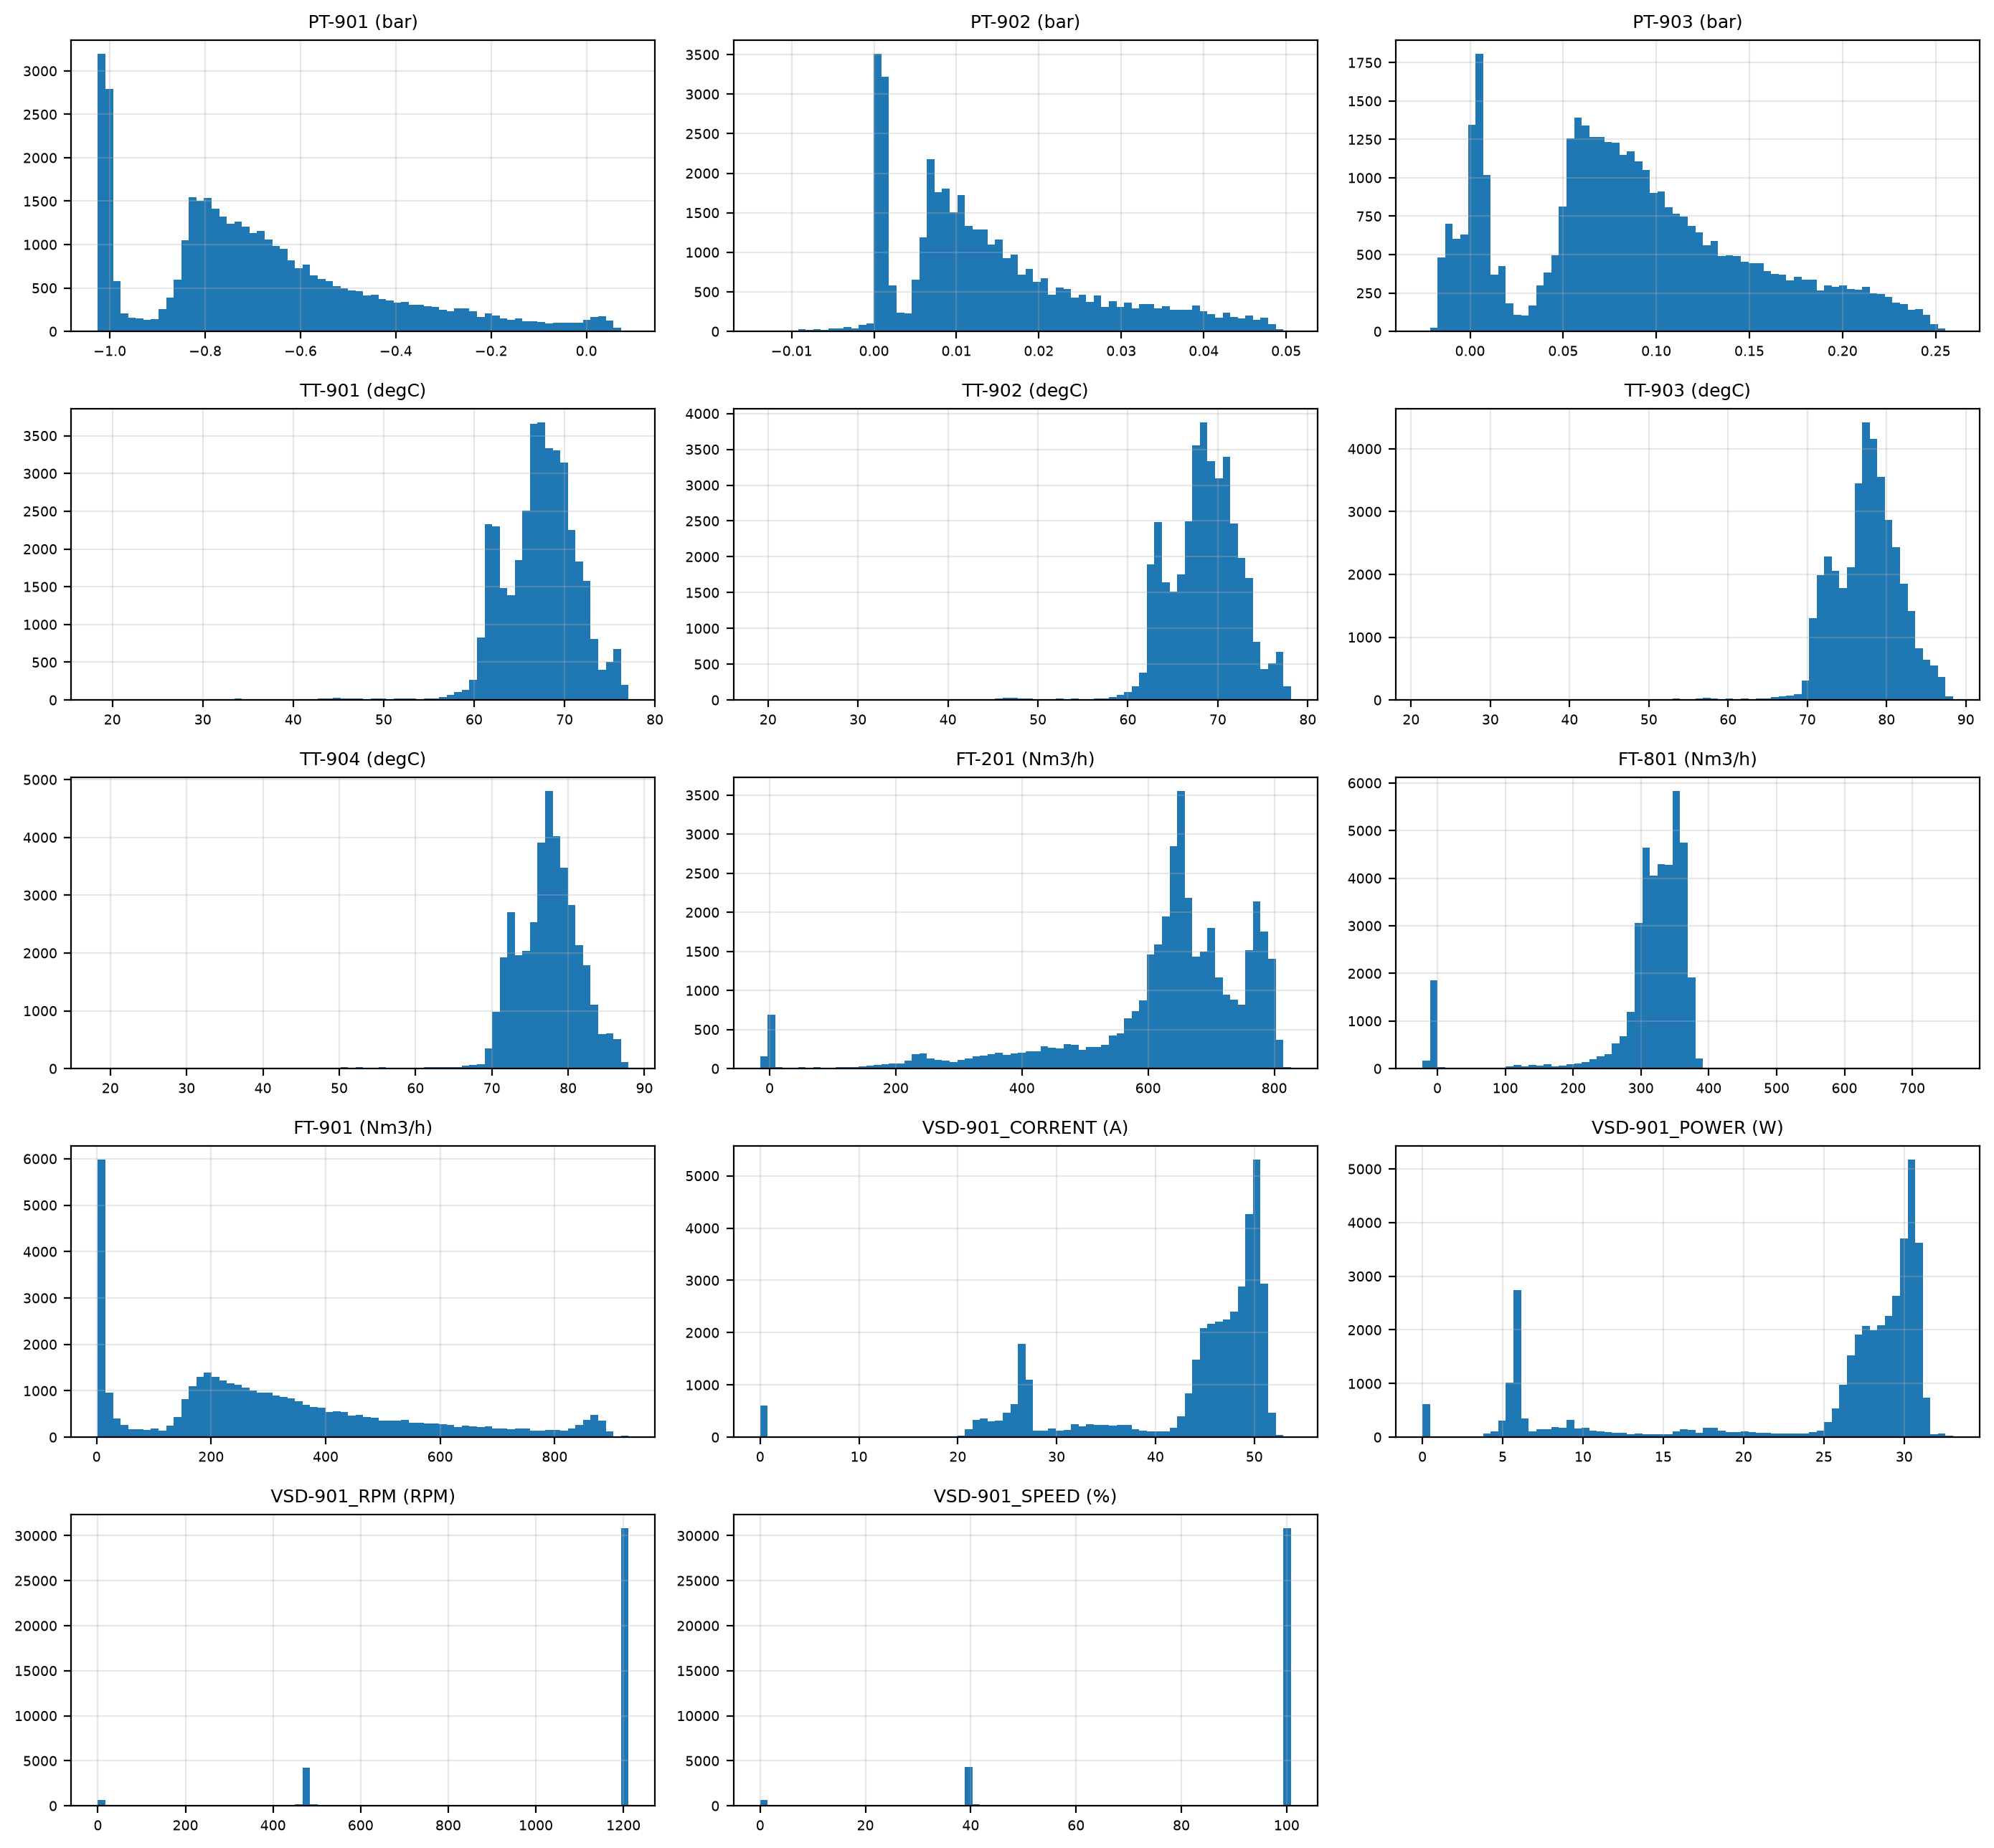
\includegraphics[width=0.98\textwidth]{imgs/eda_appendix_distributions.png}
    \caption{Distributions of the fourteen continuous process variables over the full
    collection period.}
    \label{fig:ap1_distributions}
\end{figure}

\section{Correlation Matrix Values} \label{ap1:correlation}

Table~\ref{tab:ap1_correlation} reports the numerical Pearson correlation coefficients
underlying the matrix shown in Figure~\ref{fig:eda_correlation}. As in the figure, the
coefficients are computed over the plant's production modes only (Mode 8 and 9), and the
frozen PT-903 episode and the FT-801 sentinel readings are excluded, since a constant
reading carries no variance and would distort every coefficient involving the affected
variable.

These values are what motivates the correlation thresholds used when propagating an
injected fault to physically related sensors, described in
Section~\ref{sec:fault_single}.

\begin{table}[htbp]
\centering
\caption{Pearson correlation coefficients between the continuous process variables,
restricted to production modes (Mode 8 and 9).}
\label{tab:ap1_correlation}
\tiny
% Auto-generated by eda.ipynb -- do not edit by hand
\begin{tabular}{lrrrrrrrrrrrrrr}
\hline
 & \rotatebox{90}{PT-901} & \rotatebox{90}{PT-902} & \rotatebox{90}{PT-903} & \rotatebox{90}{TT-901} & \rotatebox{90}{TT-902} & \rotatebox{90}{TT-903} & \rotatebox{90}{TT-904} & \rotatebox{90}{FT-201} & \rotatebox{90}{FT-801} & \rotatebox{90}{FT-901} & \rotatebox{90}{VSD-901\_CORRENT} & \rotatebox{90}{VSD-901\_POWER} & \rotatebox{90}{VSD-901\_RPM} & \rotatebox{90}{VSD-901\_SPEED} \\
\hline
PT-901 & 1.00 & 0.96 & 0.94 & -0.03 & -0.02 & -0.11 & -0.15 & 0.04 & 0.07 & 0.74 & 0.61 & 0.52 & 0.36 & 0.34 \\
PT-902 & 0.96 & 1.00 & 0.97 & -0.06 & -0.05 & -0.14 & -0.19 & 0.08 & 0.08 & 0.85 & 0.62 & 0.56 & 0.40 & 0.39 \\
PT-903 & 0.94 & 0.97 & 1.00 & -0.00 & 0.01 & -0.10 & -0.13 & 0.11 & 0.05 & 0.88 & 0.74 & 0.68 & 0.51 & 0.50 \\
TT-901 & -0.03 & -0.06 & -0.00 & 1.00 & 1.00 & 0.94 & 0.97 & 0.01 & -0.01 & -0.02 & 0.11 & 0.14 & 0.16 & 0.16 \\
TT-902 & -0.02 & -0.05 & 0.01 & 1.00 & 1.00 & 0.94 & 0.97 & -0.00 & -0.01 & -0.01 & 0.11 & 0.14 & 0.16 & 0.16 \\
TT-903 & -0.11 & -0.14 & -0.10 & 0.94 & 0.94 & 1.00 & 0.98 & -0.13 & -0.08 & -0.14 & -0.05 & -0.01 & 0.04 & 0.04 \\
TT-904 & -0.15 & -0.19 & -0.13 & 0.97 & 0.97 & 0.98 & 1.00 & -0.05 & -0.07 & -0.15 & 0.03 & 0.08 & 0.13 & 0.13 \\
FT-201 & 0.04 & 0.08 & 0.11 & 0.01 & -0.00 & -0.13 & -0.05 & 1.00 & 0.58 & 0.25 & 0.31 & 0.36 & 0.41 & 0.42 \\
FT-801 & 0.07 & 0.08 & 0.05 & -0.01 & -0.01 & -0.08 & -0.07 & 0.58 & 1.00 & 0.04 & 0.02 & 0.01 & -0.01 & -0.01 \\
FT-901 & 0.74 & 0.85 & 0.88 & -0.02 & -0.01 & -0.14 & -0.15 & 0.25 & 0.04 & 1.00 & 0.75 & 0.72 & 0.58 & 0.57 \\
VSD-901\_CORRENT & 0.61 & 0.62 & 0.74 & 0.11 & 0.11 & -0.05 & 0.03 & 0.31 & 0.02 & 0.75 & 1.00 & 0.98 & 0.85 & 0.84 \\
VSD-901\_POWER & 0.52 & 0.56 & 0.68 & 0.14 & 0.14 & -0.01 & 0.08 & 0.36 & 0.01 & 0.72 & 0.98 & 1.00 & 0.94 & 0.93 \\
VSD-901\_RPM & 0.36 & 0.40 & 0.51 & 0.16 & 0.16 & 0.04 & 0.13 & 0.41 & -0.01 & 0.58 & 0.85 & 0.94 & 1.00 & 1.00 \\
VSD-901\_SPEED & 0.34 & 0.39 & 0.50 & 0.16 & 0.16 & 0.04 & 0.13 & 0.42 & -0.01 & 0.57 & 0.84 & 0.93 & 1.00 & 1.00 \\
\hline
\end{tabular}

\end{table}

\section{Production Sessions} \label{ap1:sessions}

Figures~\ref{fig:ap1_session_1} to~\ref{fig:ap1_session_17} present each of the eleven
production sessions retained after data cleaning
(Table~\ref{tab:cleaning_sessions}) individually, with the variables grouped by
measurement type. Unlike the figures in Section~\ref{ap1:timeseries}, these correspond to
the cleaned data: restricted to production modes, resampled to a strict one-minute
frequency, and with short gaps filled by linear interpolation.

Sessions 16 and 17 are the two used for fault injection
(Section~\ref{sec:fault_scenarios}); the figures shown here correspond to their original,
fault-free state, prior to any injection.

Table~\ref{tab:ap1_session_stats} summarises the mean value of a representative subset of
the variables within each session. The variation across sessions is modest, which is
consistent with the plant operating under nominal conditions throughout the collection
period, and supports the assumption stated in Section~\ref{sec:data_acquisition}.

\begin{table}[htbp]
\centering
\caption{Per-session mean values of a representative subset of the process variables.}
\label{tab:ap1_session_stats}
\small
% Auto-generated by eda.ipynb -- do not edit by hand
\begin{tabular}{crrrrr}
\hline
\textbf{Session} & \textbf{Obs.} & \textbf{PT-903 mean} & \textbf{TT-901 mean} & \textbf{TT-904 mean} & \textbf{VSD current mean} \\
\hline
1 & 2,900 & 0.086 & 72.01 & 82.39 & 44.03 \\
2 & 1,799 & 0.088 & 73.51 & 83.75 & 44.53 \\
3 & 4,763 & 0.093 & 68.47 & 78.64 & 43.57 \\
5 & 1,606 & 0.089 & 65.49 & 76.28 & 44.35 \\
8 & 1,235 & 0.094 & 68.13 & 78.69 & 44.77 \\
12 & 2,556 & 0.090 & 68.82 & 78.12 & 44.10 \\
13 & 8,938 & 0.089 & 68.67 & 78.50 & 44.20 \\
14 & 2,527 & 0.099 & 63.92 & 73.55 & 42.99 \\
15 & 3,270 & 0.083 & 68.24 & 78.40 & 44.03 \\
16 & 3,367 & 0.082 & 62.50 & 72.17 & 41.99 \\
17 & 4,415 & 0.036 & 62.32 & 72.75 & 42.81 \\
\hline
\textbf{Total} & \textbf{37,376} & & & & \\
\hline
\end{tabular}

\end{table}

\begin{figure}[htbp]
    \centering
    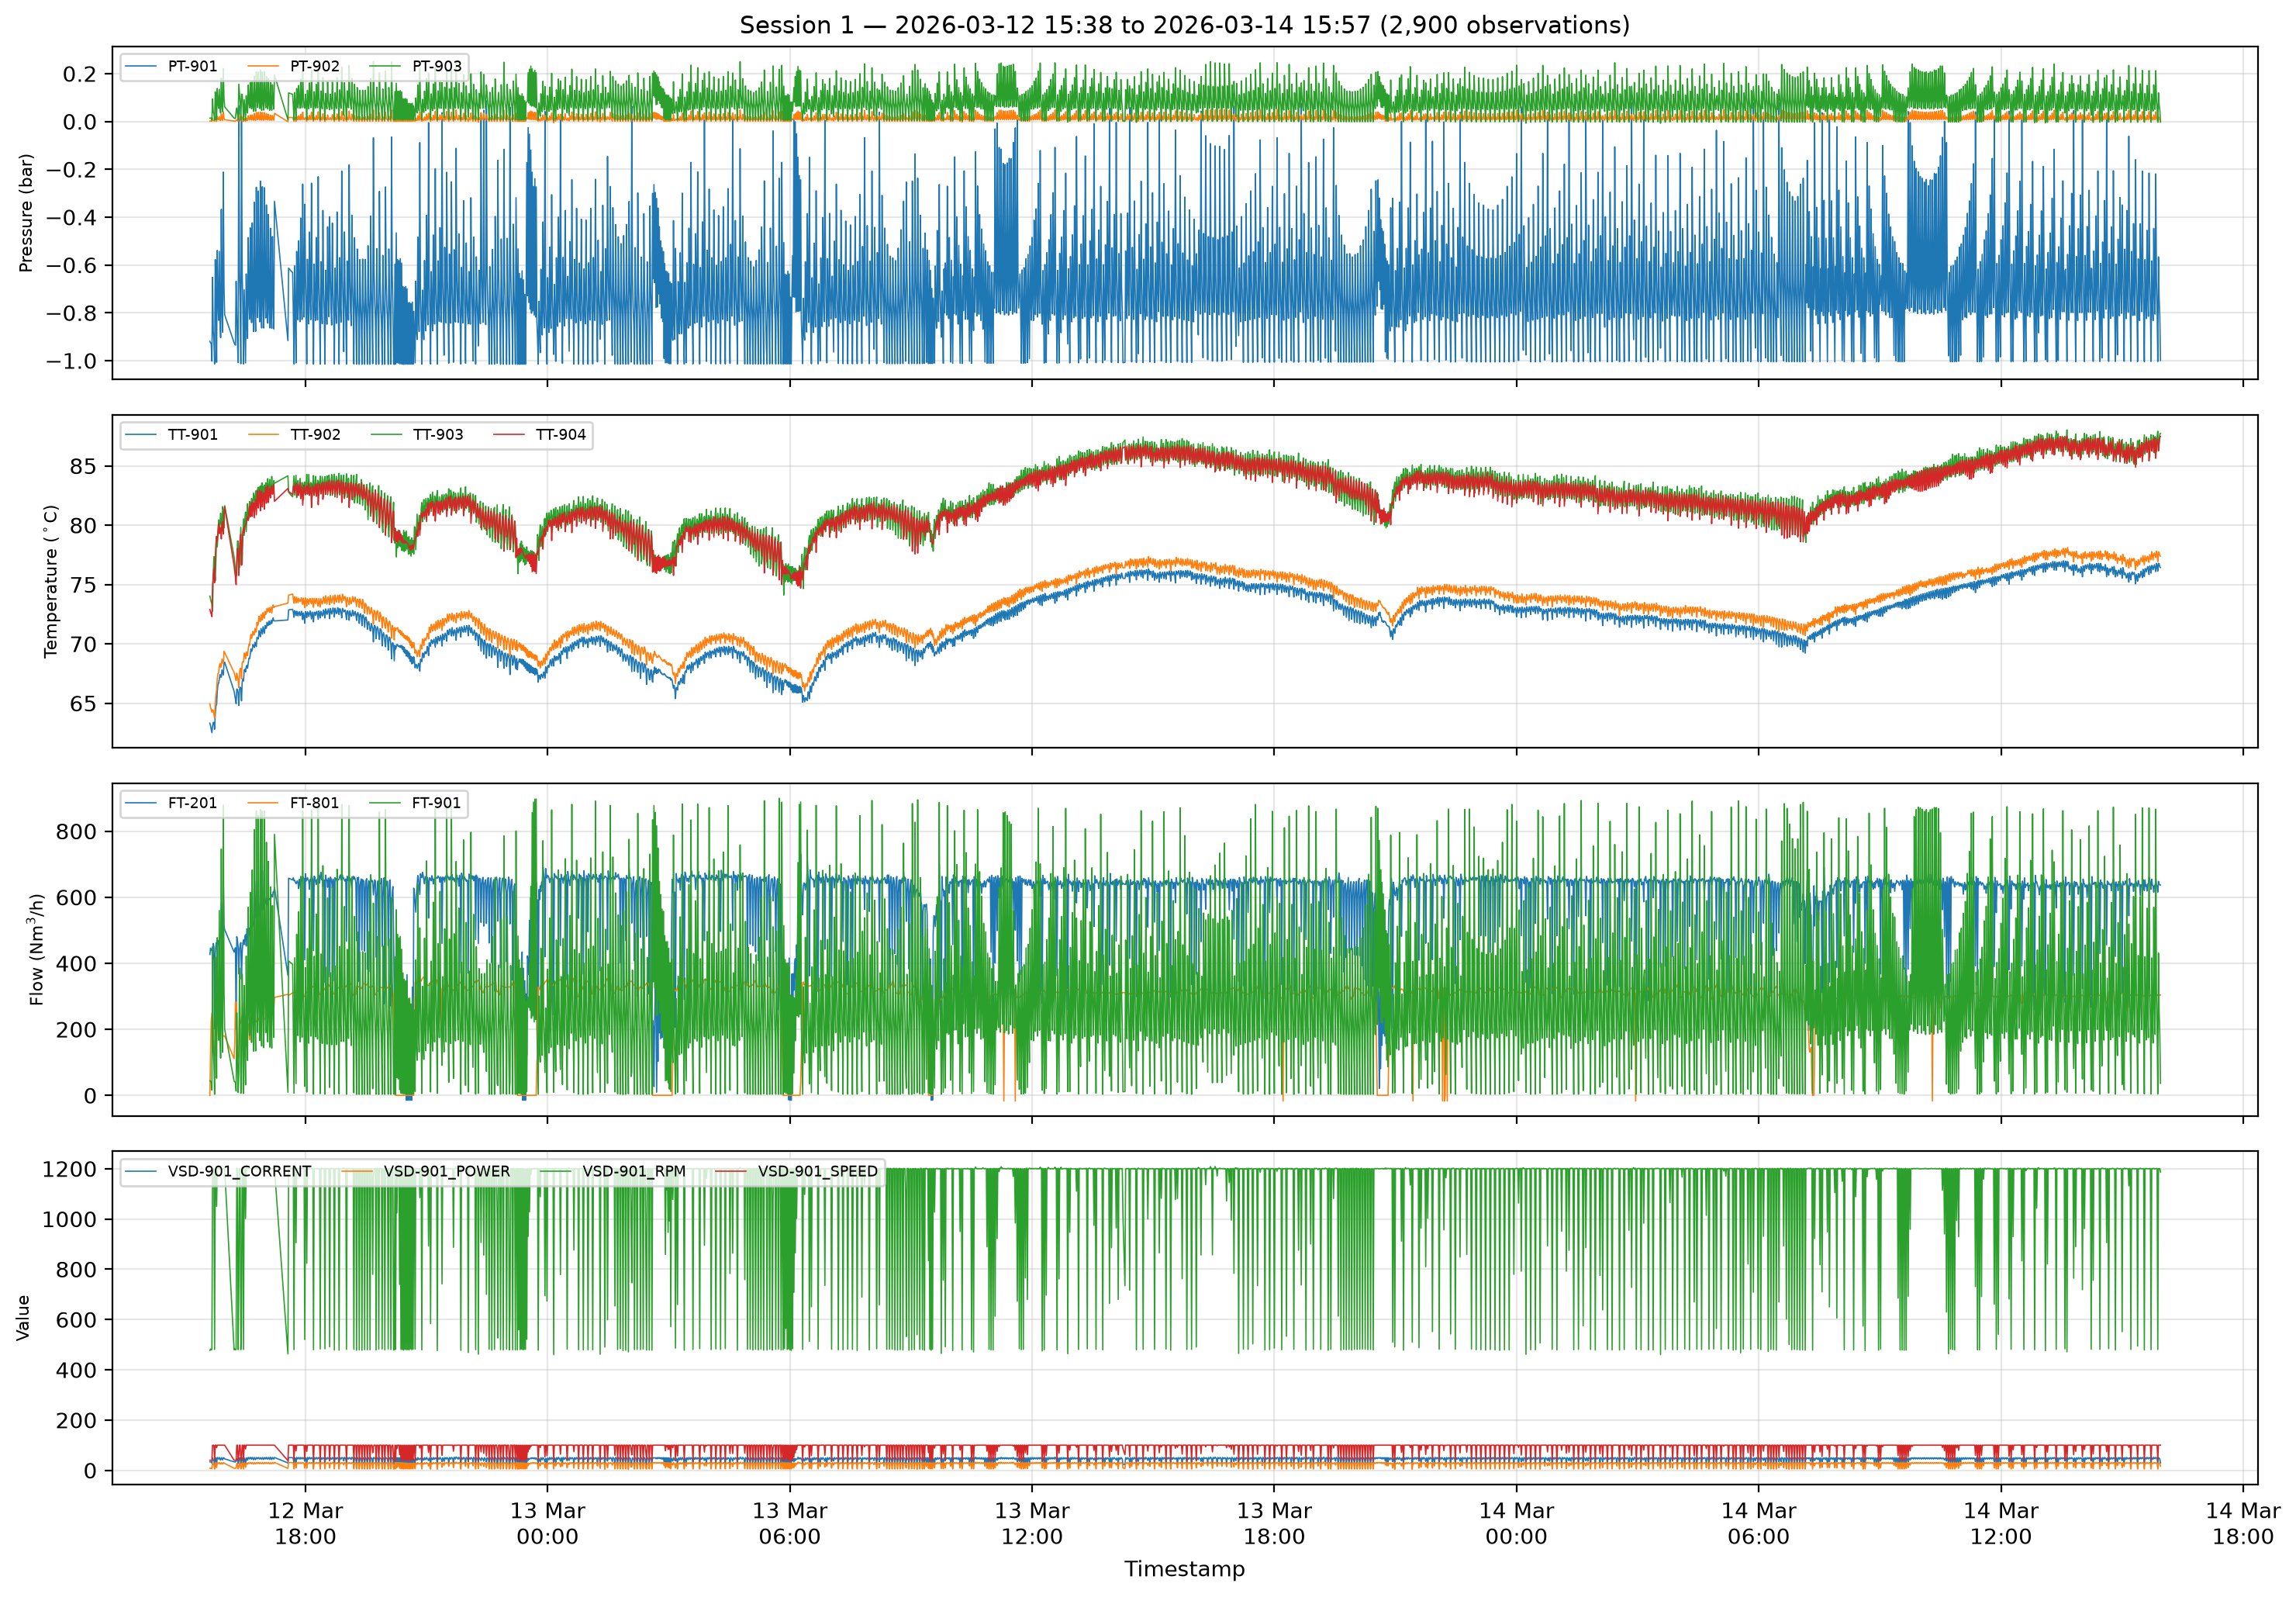
\includegraphics[width=0.95\textwidth]{imgs/eda_appendix_session_1.png}
    \caption{Session 1 (2026-03-12 15:38 to 2026-03-14 15:57, 2{,}900 observations).}
    \label{fig:ap1_session_1}
\end{figure}

\begin{figure}[htbp]
    \centering
    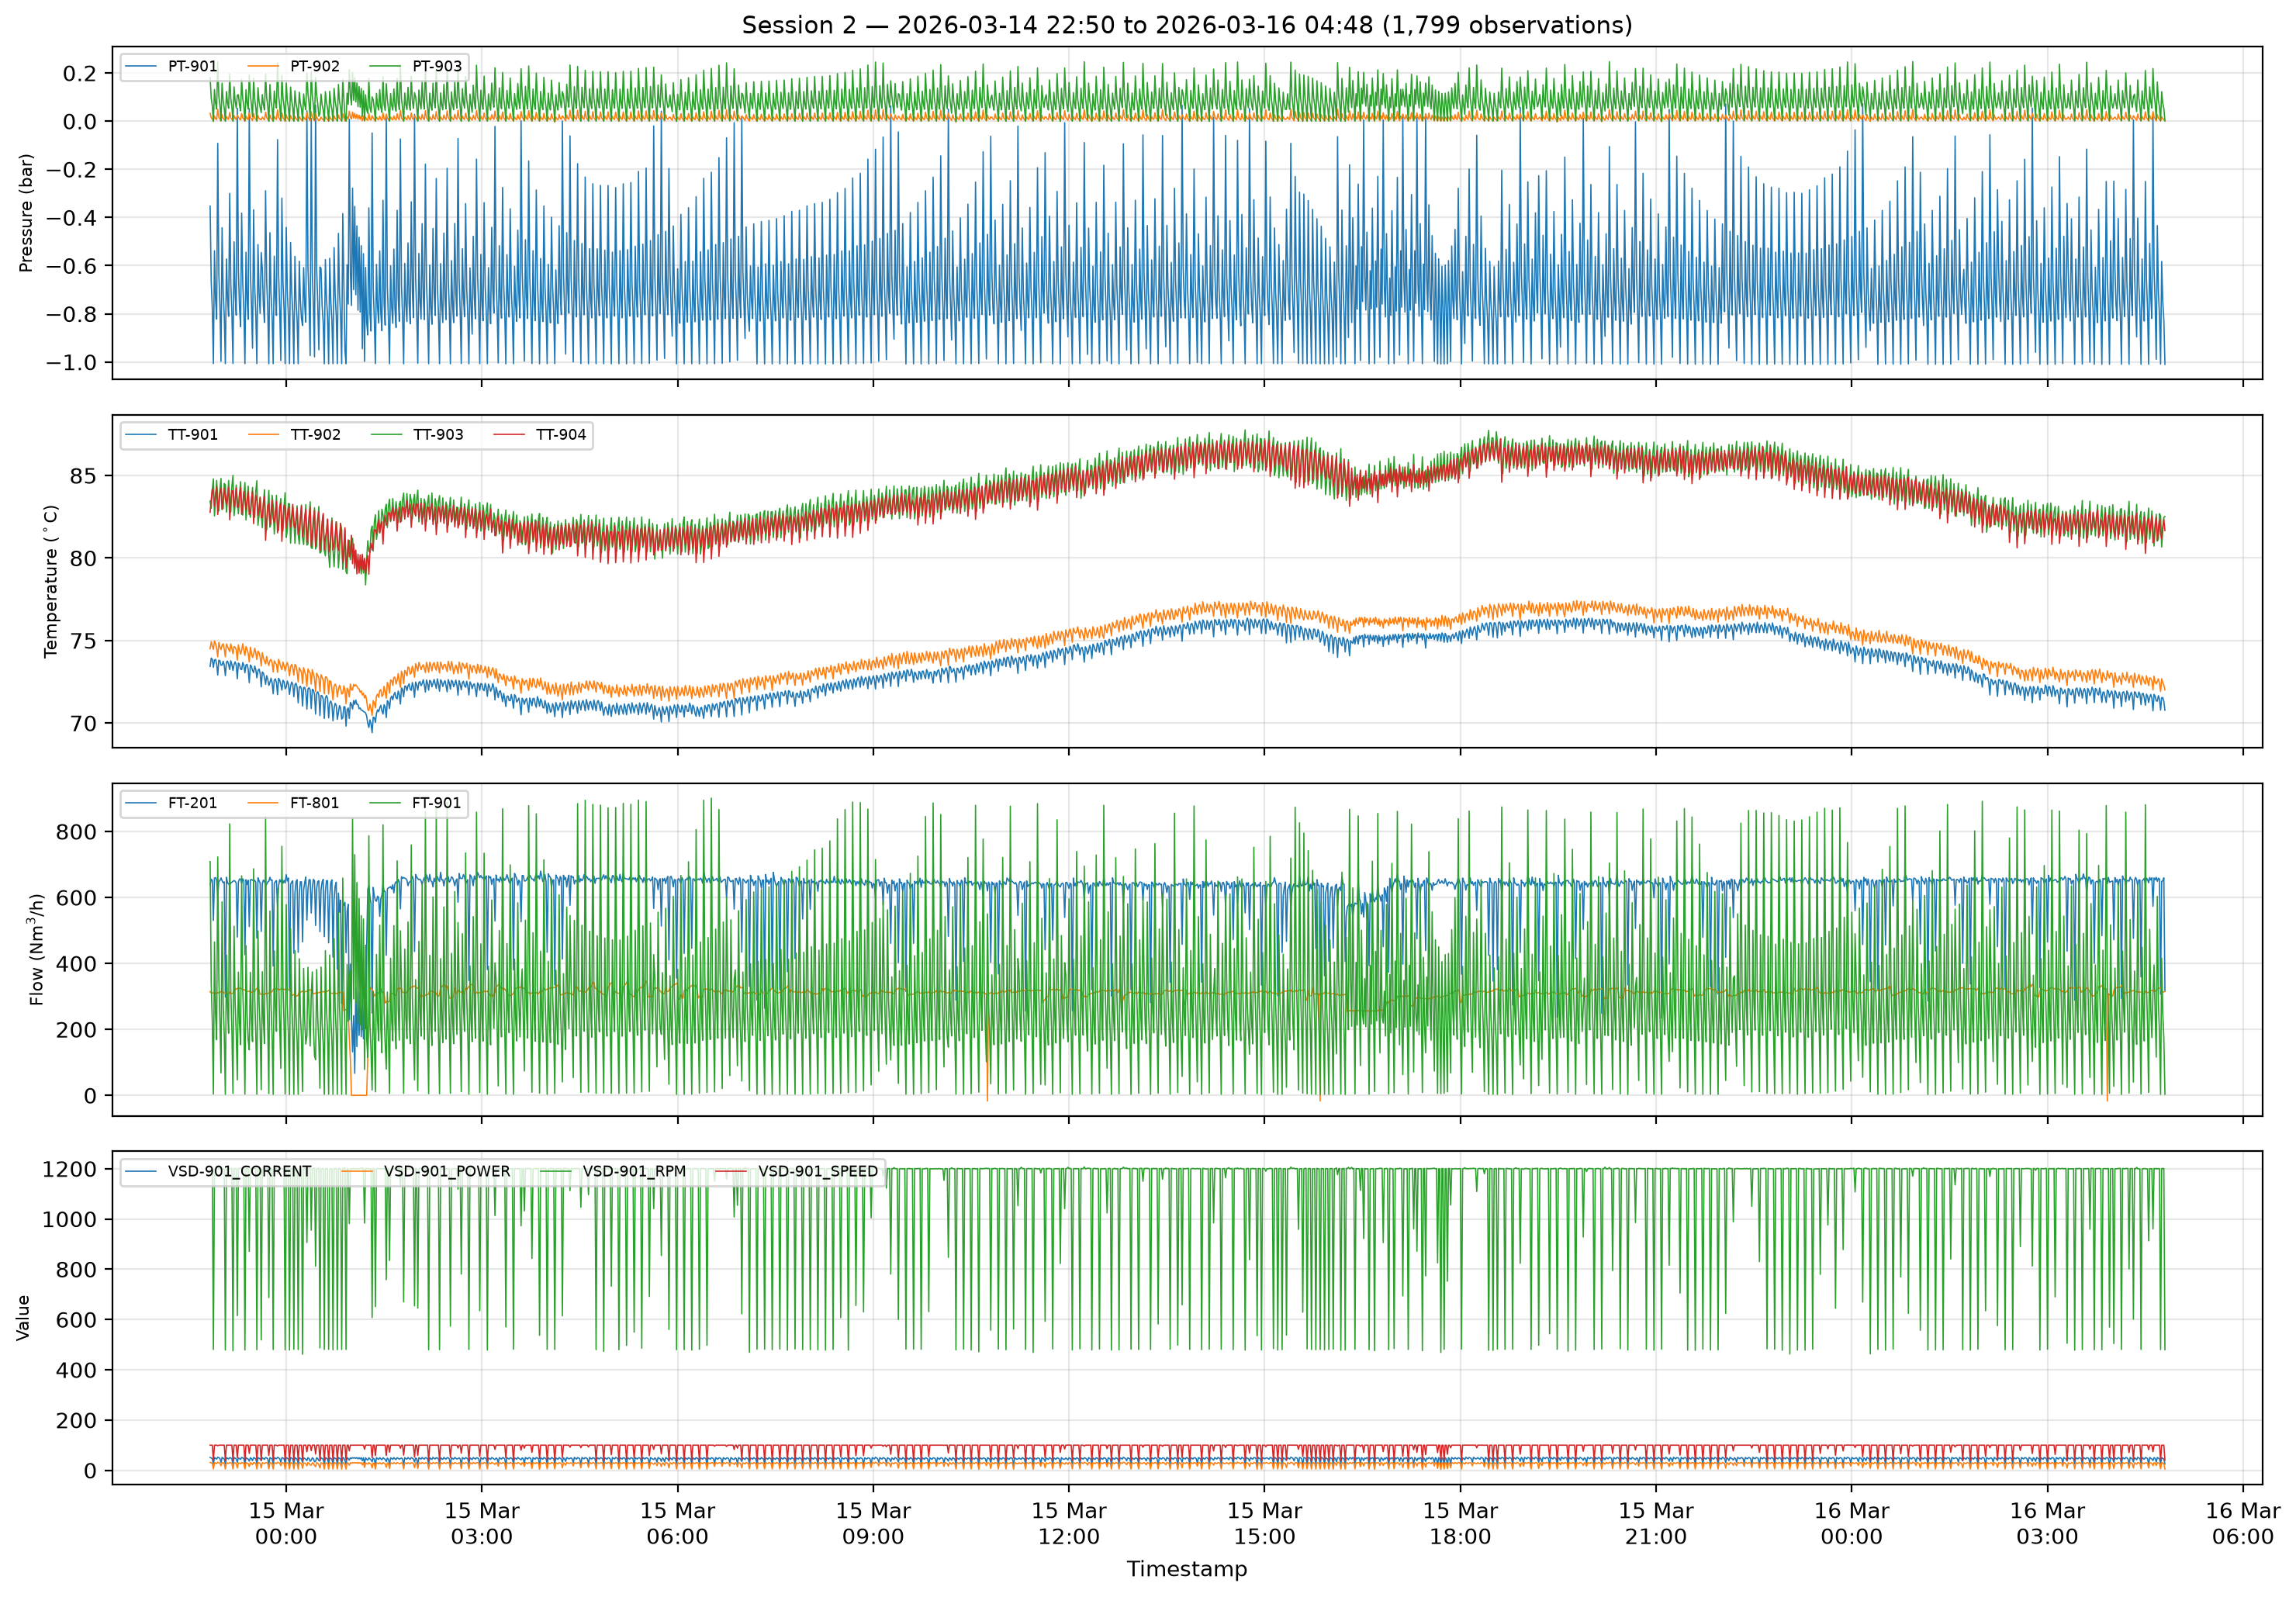
\includegraphics[width=0.95\textwidth]{imgs/eda_appendix_session_2.png}
    \caption{Session 2 (2026-03-14 22:50 to 2026-03-16 04:48, 1{,}799 observations).}
    \label{fig:ap1_session_2}
\end{figure}

\begin{figure}[htbp]
    \centering
    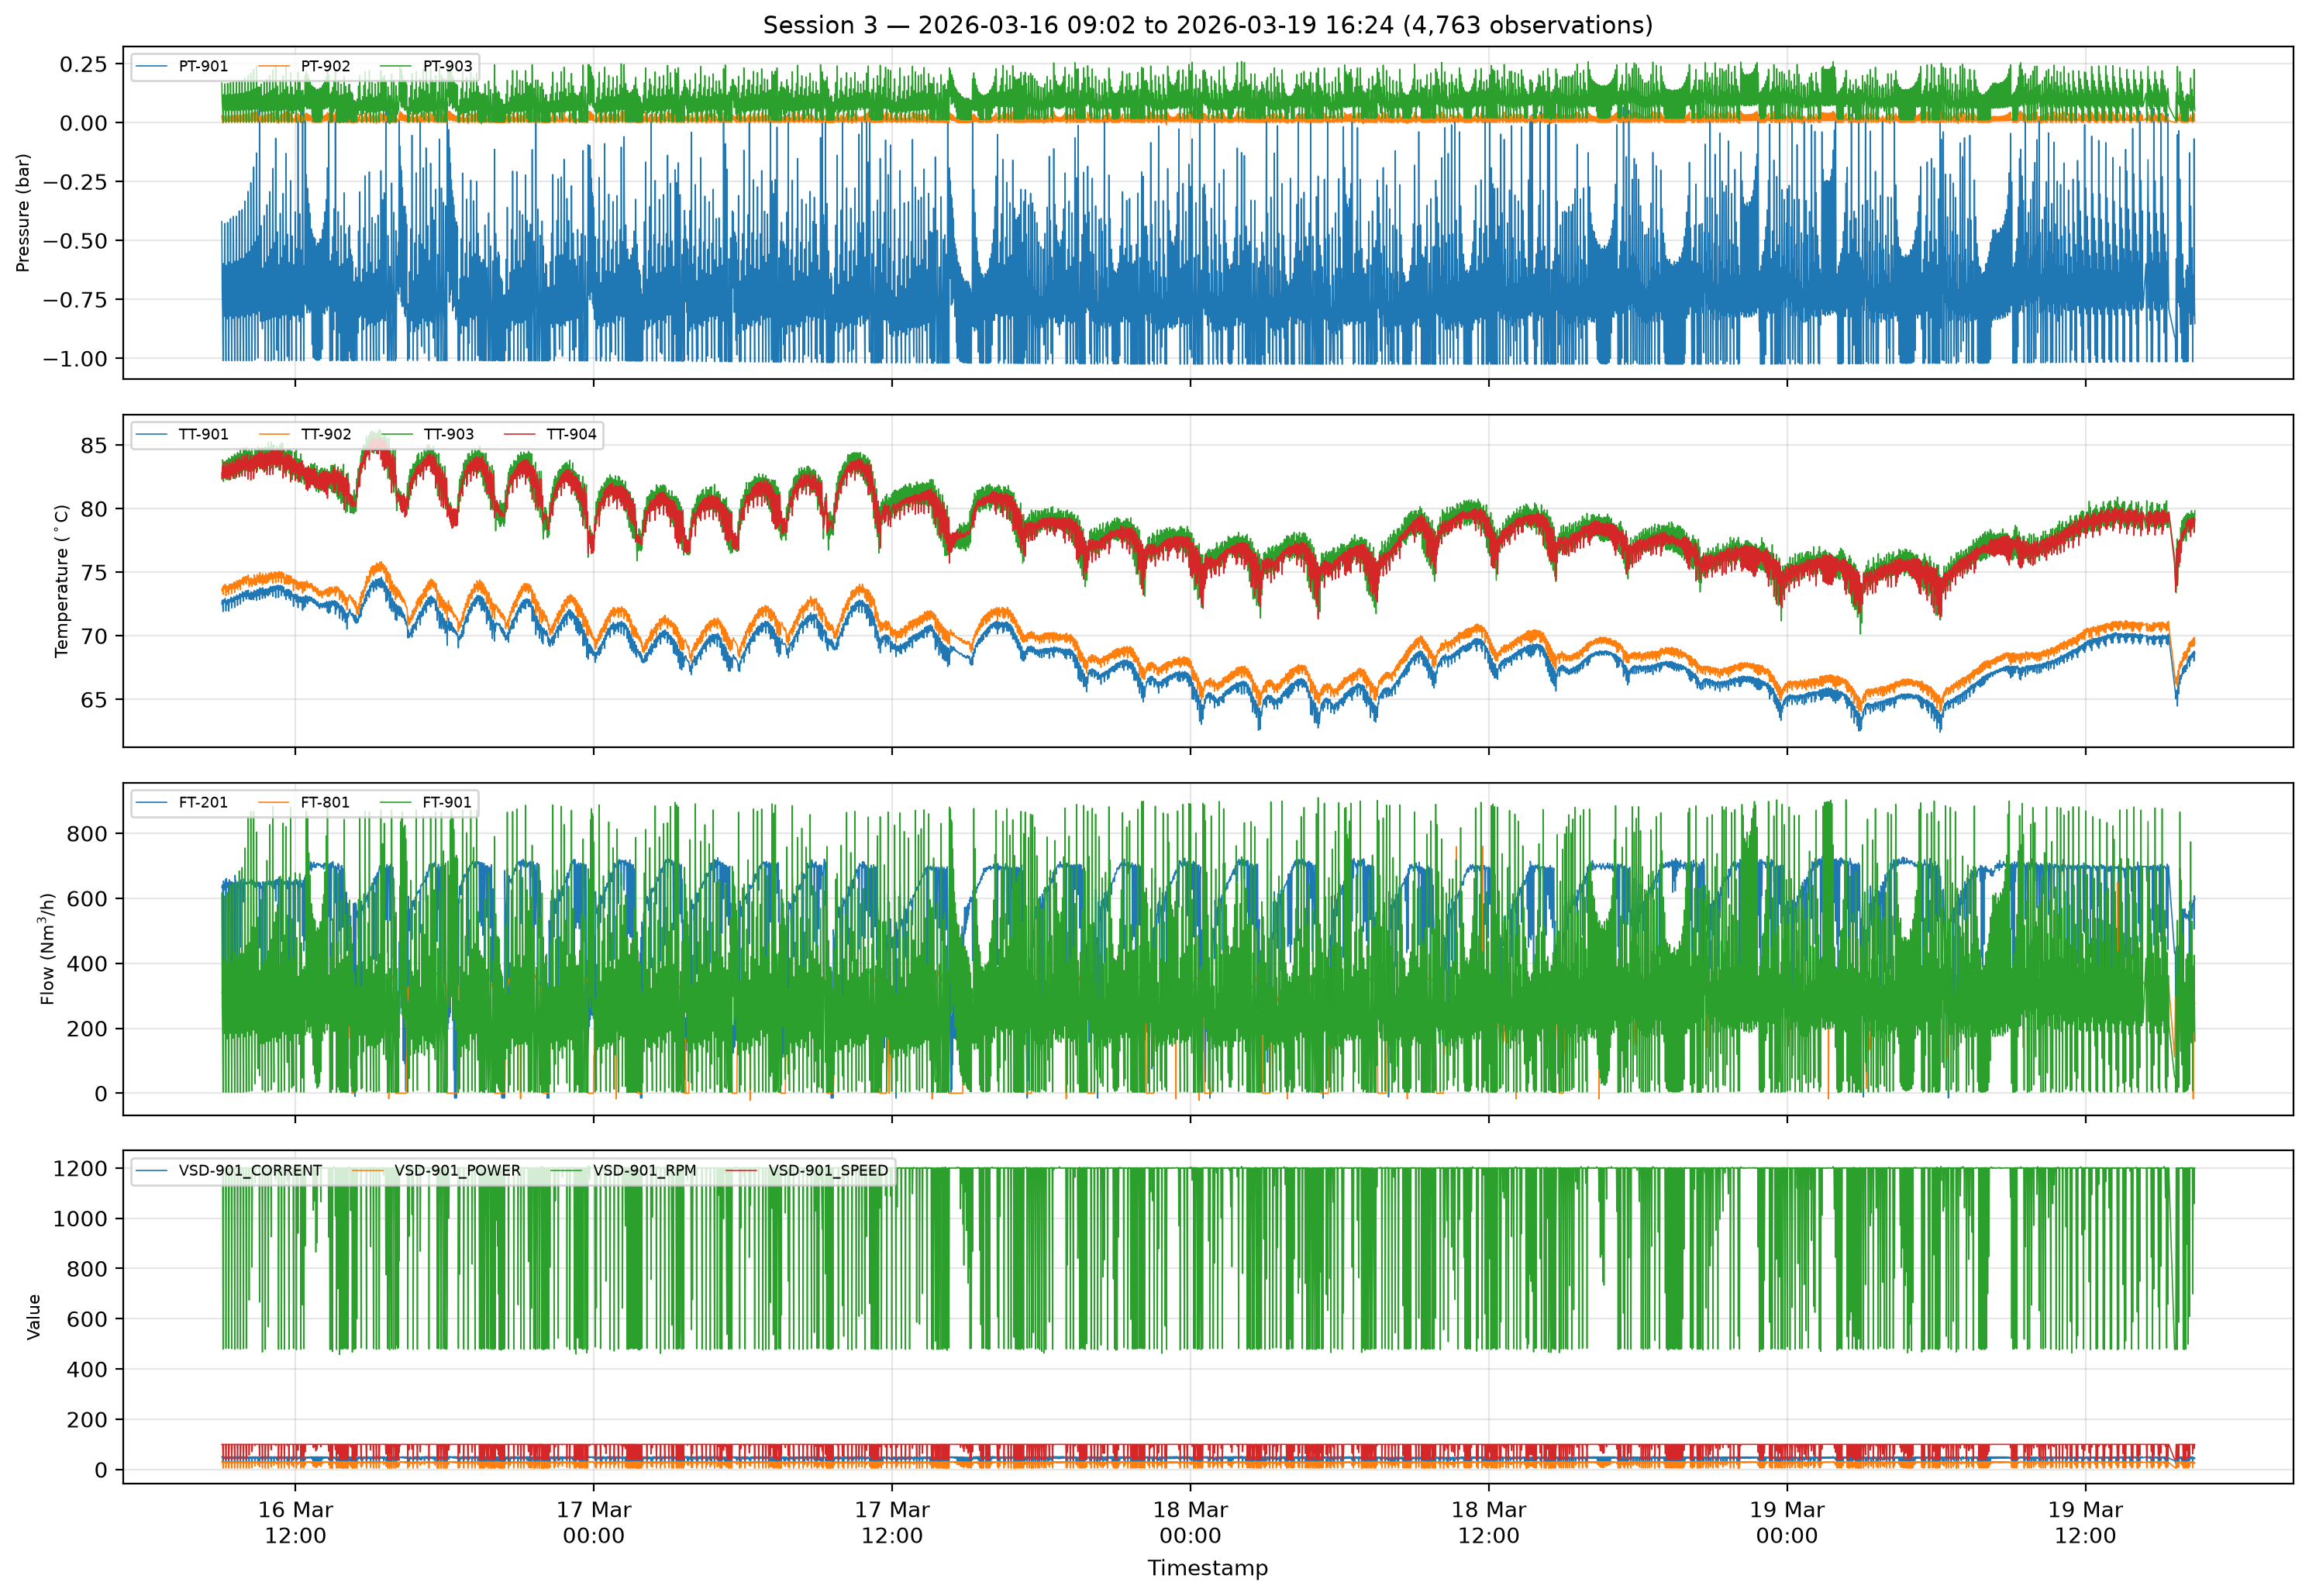
\includegraphics[width=0.95\textwidth]{imgs/eda_appendix_session_3.png}
    \caption{Session 3 (2026-03-16 09:02 to 2026-03-19 16:24, 4{,}763 observations).}
    \label{fig:ap1_session_3}
\end{figure}

\begin{figure}[htbp]
    \centering
    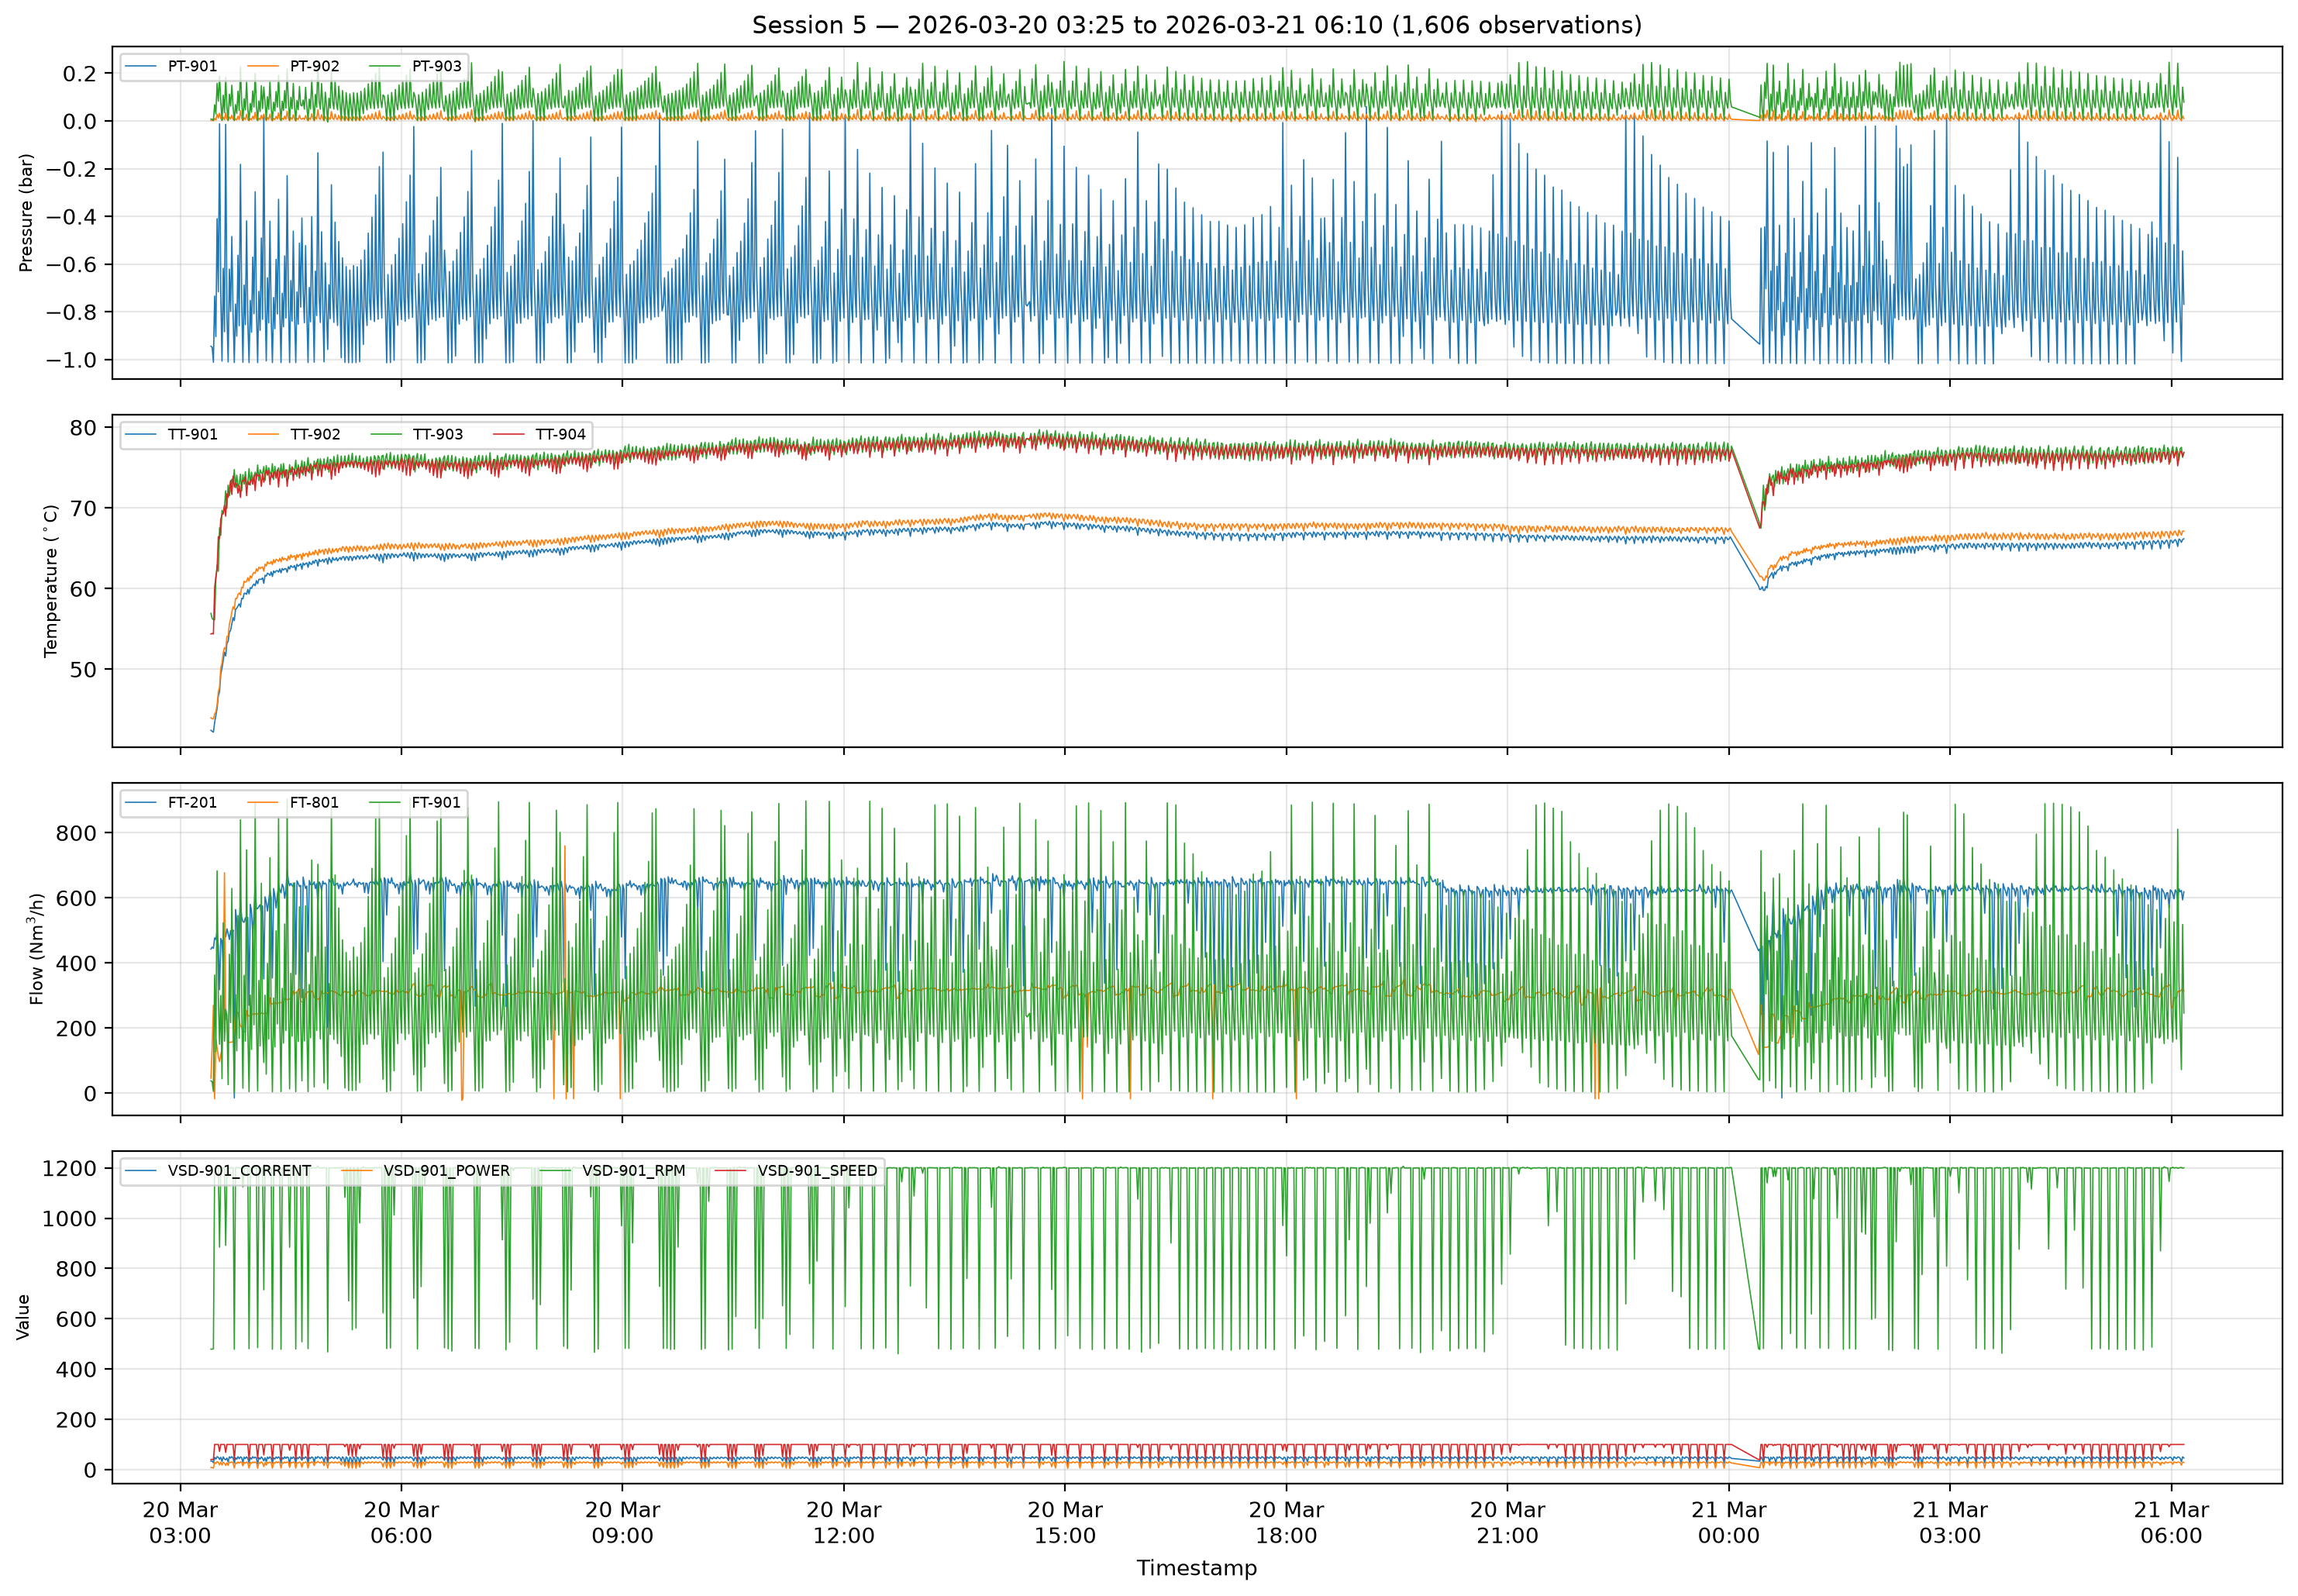
\includegraphics[width=0.95\textwidth]{imgs/eda_appendix_session_5.png}
    \caption{Session 5 (2026-03-20 03:25 to 2026-03-21 06:10, 1{,}606 observations).}
    \label{fig:ap1_session_5}
\end{figure}

\begin{figure}[htbp]
    \centering
    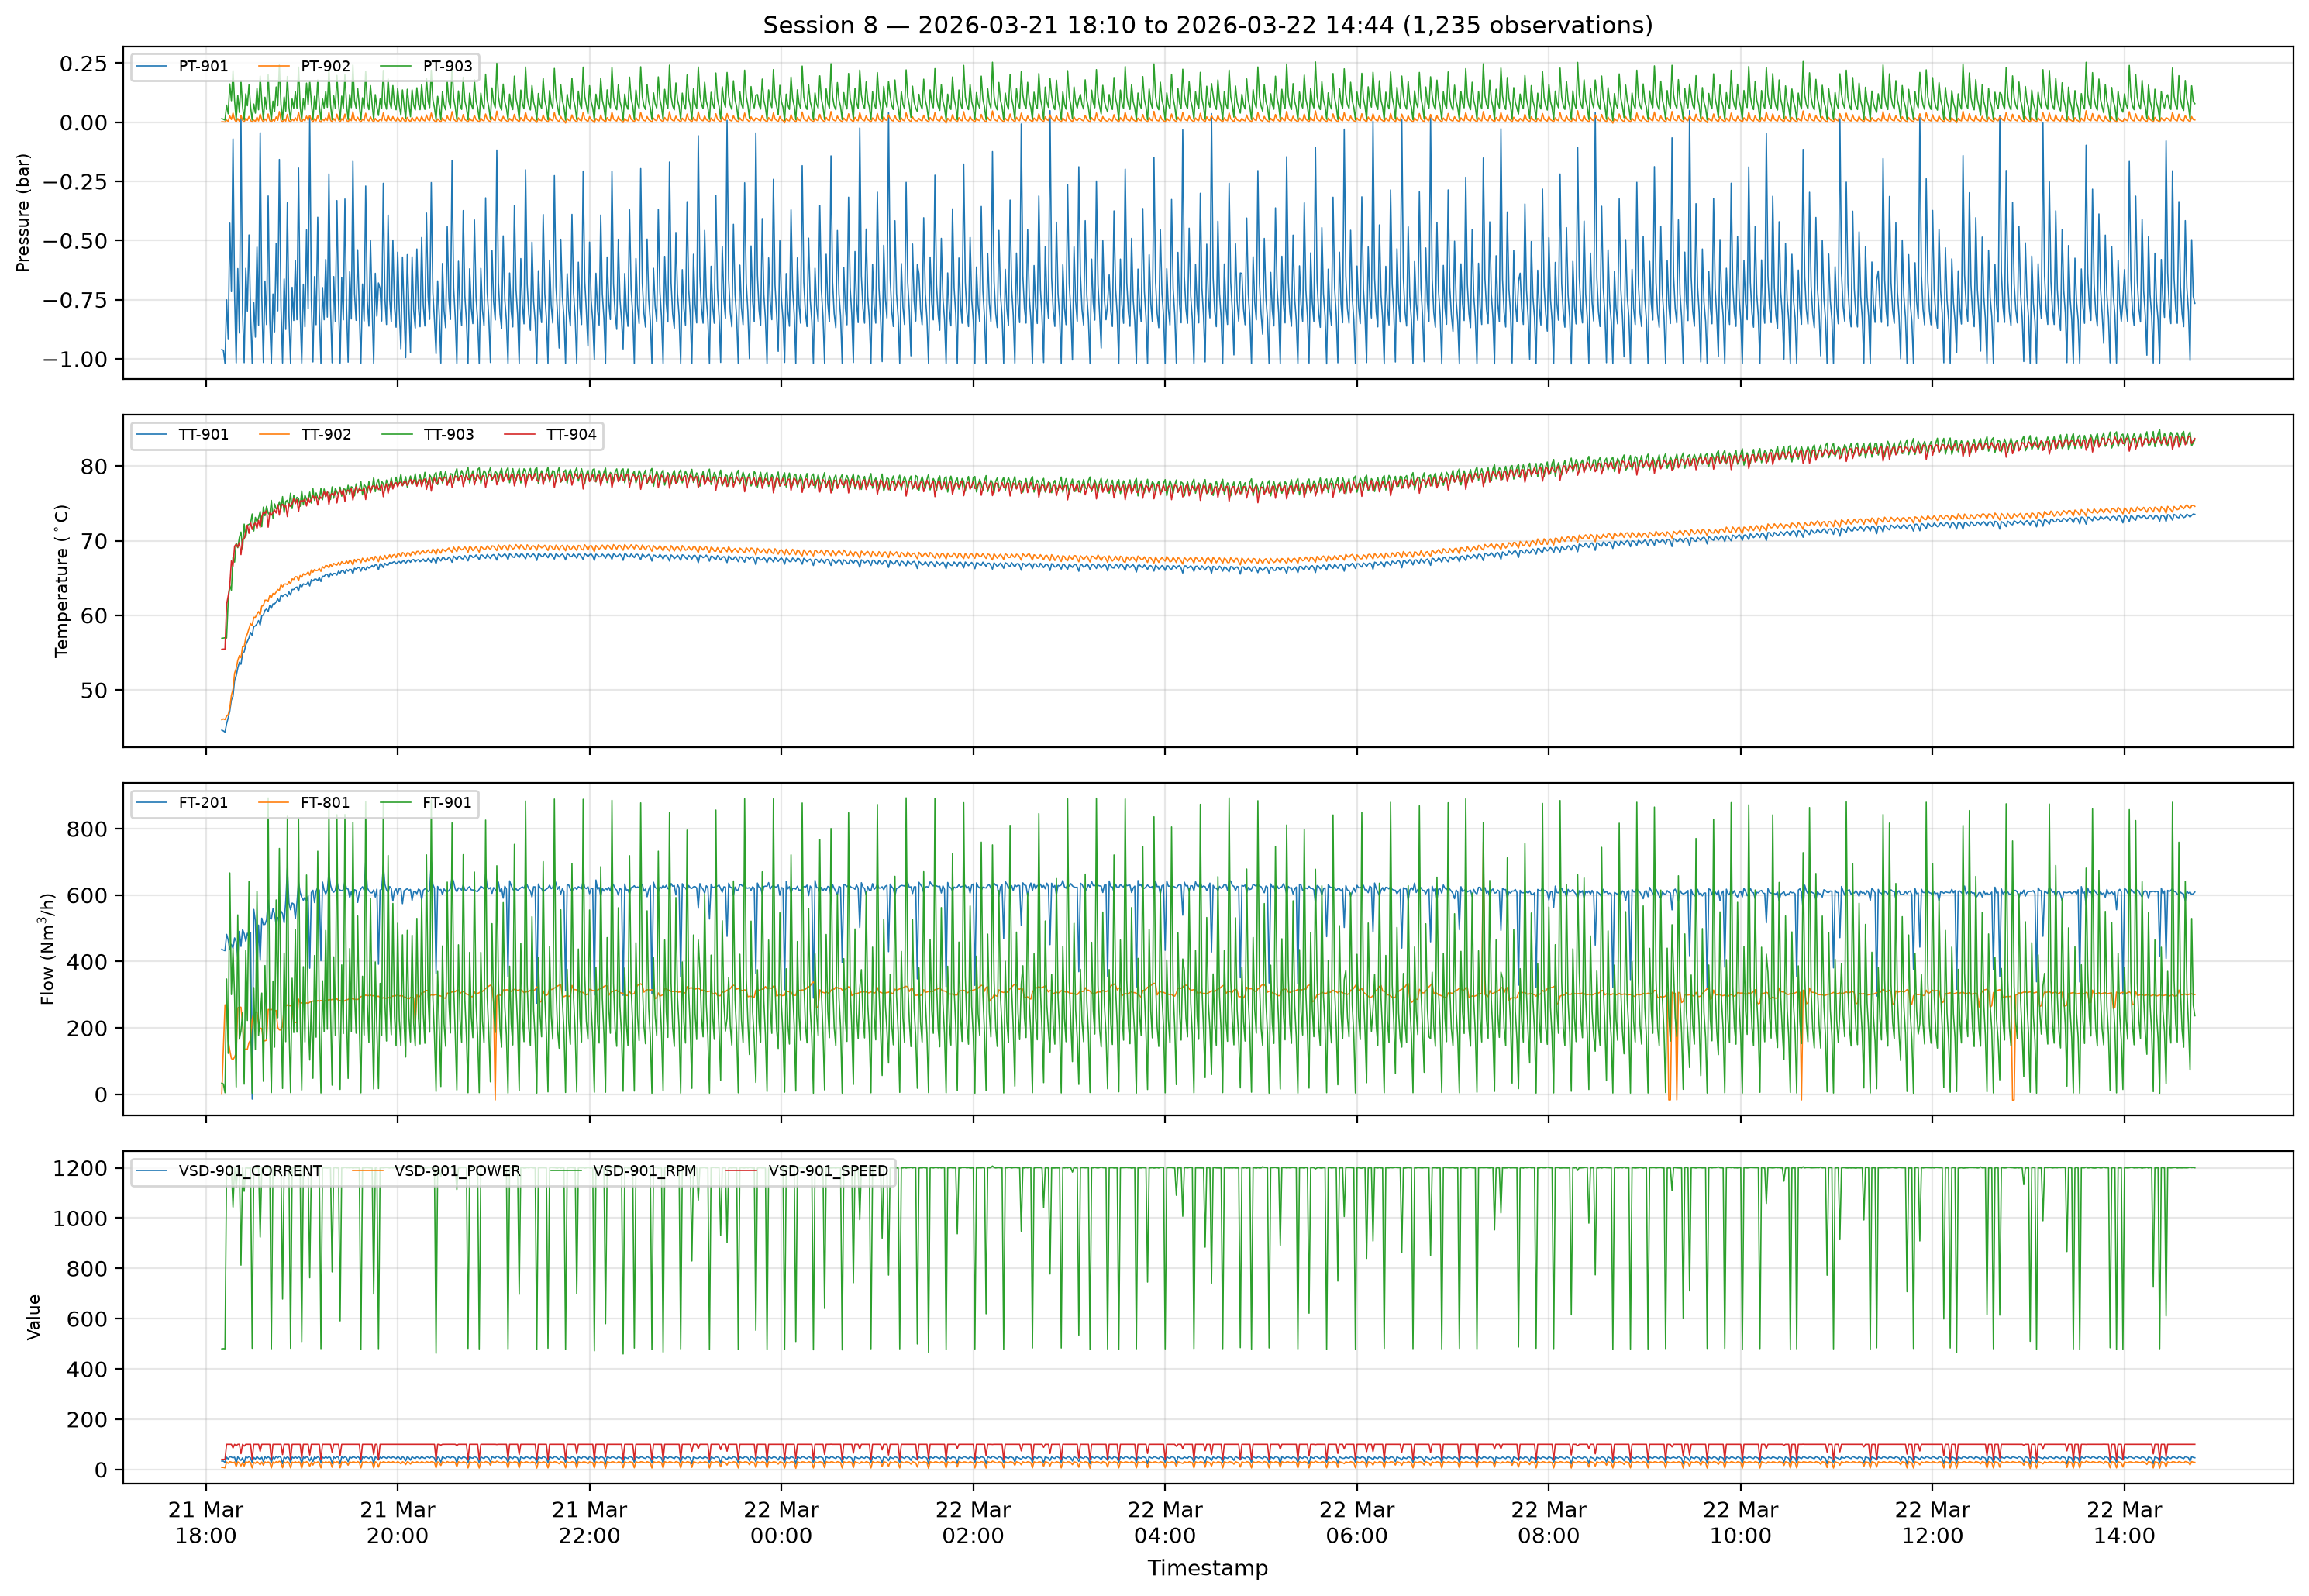
\includegraphics[width=0.95\textwidth]{imgs/eda_appendix_session_8.png}
    \caption{Session 8 (2026-03-21 18:10 to 2026-03-22 14:44, 1{,}235 observations).}
    \label{fig:ap1_session_8}
\end{figure}

\begin{figure}[htbp]
    \centering
    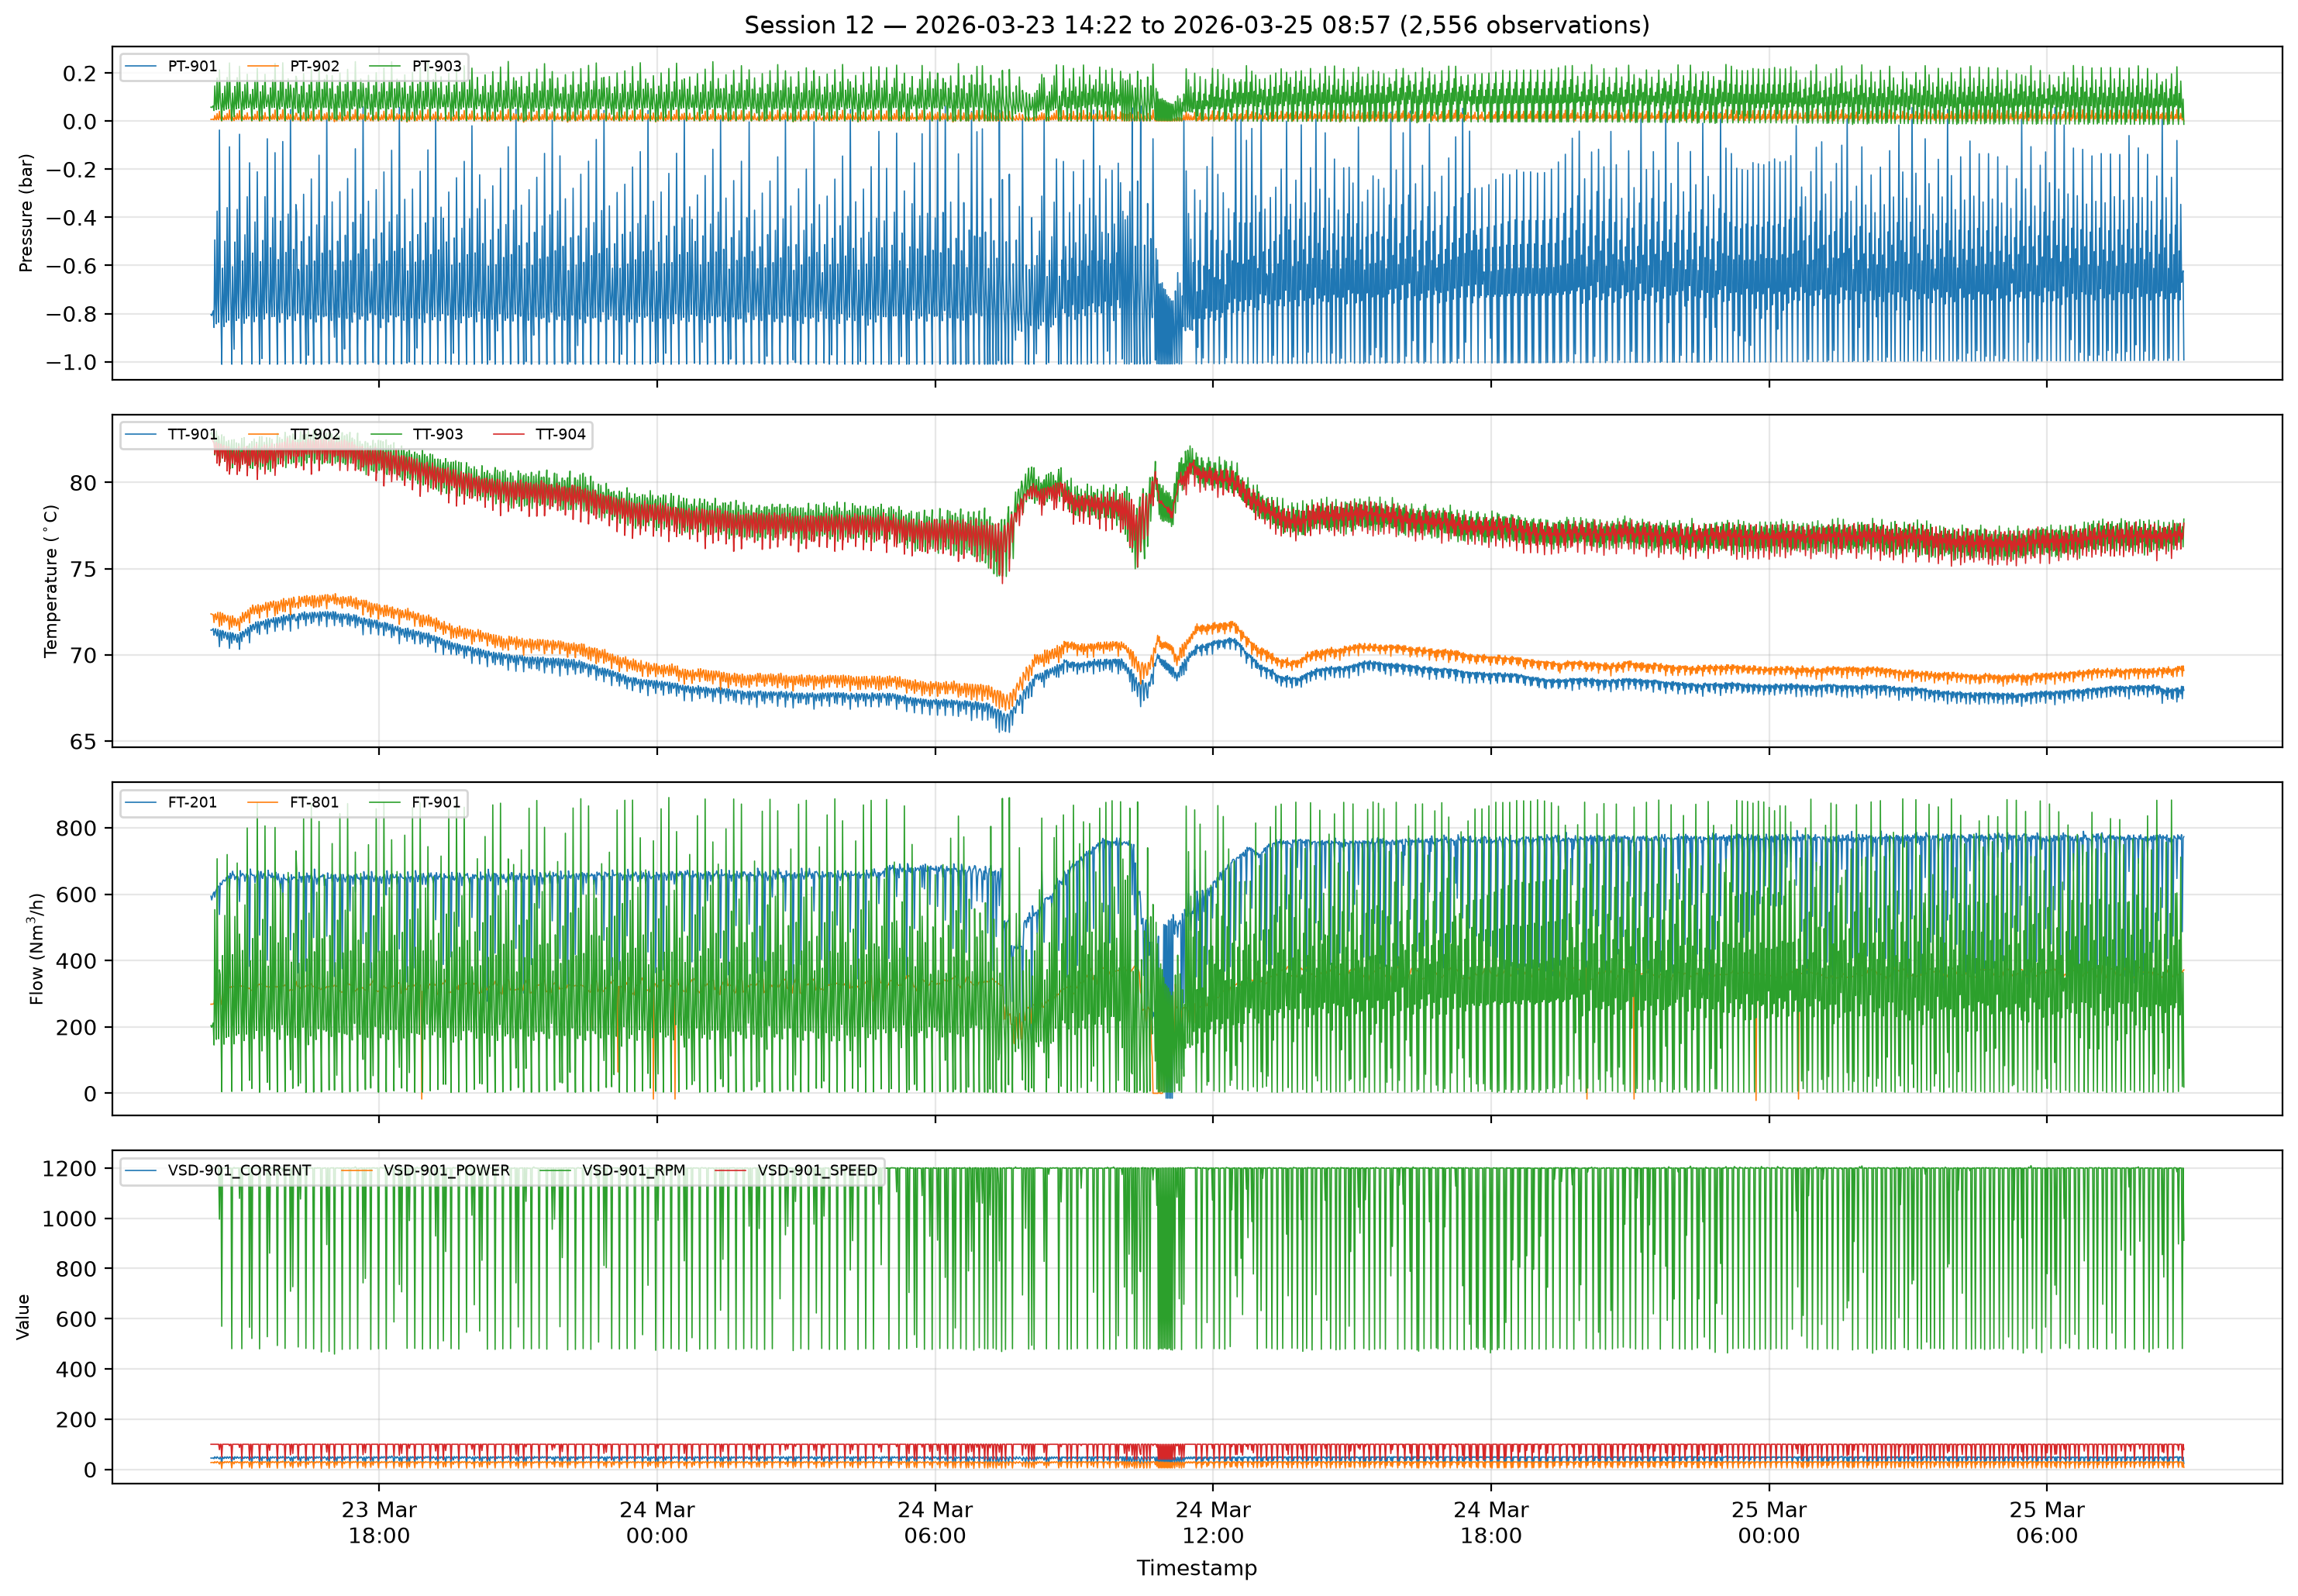
\includegraphics[width=0.95\textwidth]{imgs/eda_appendix_session_12.png}
    \caption{Session 12 (2026-03-23 14:22 to 2026-03-25 08:57, 2{,}556 observations).}
    \label{fig:ap1_session_12}
\end{figure}

\begin{figure}[htbp]
    \centering
    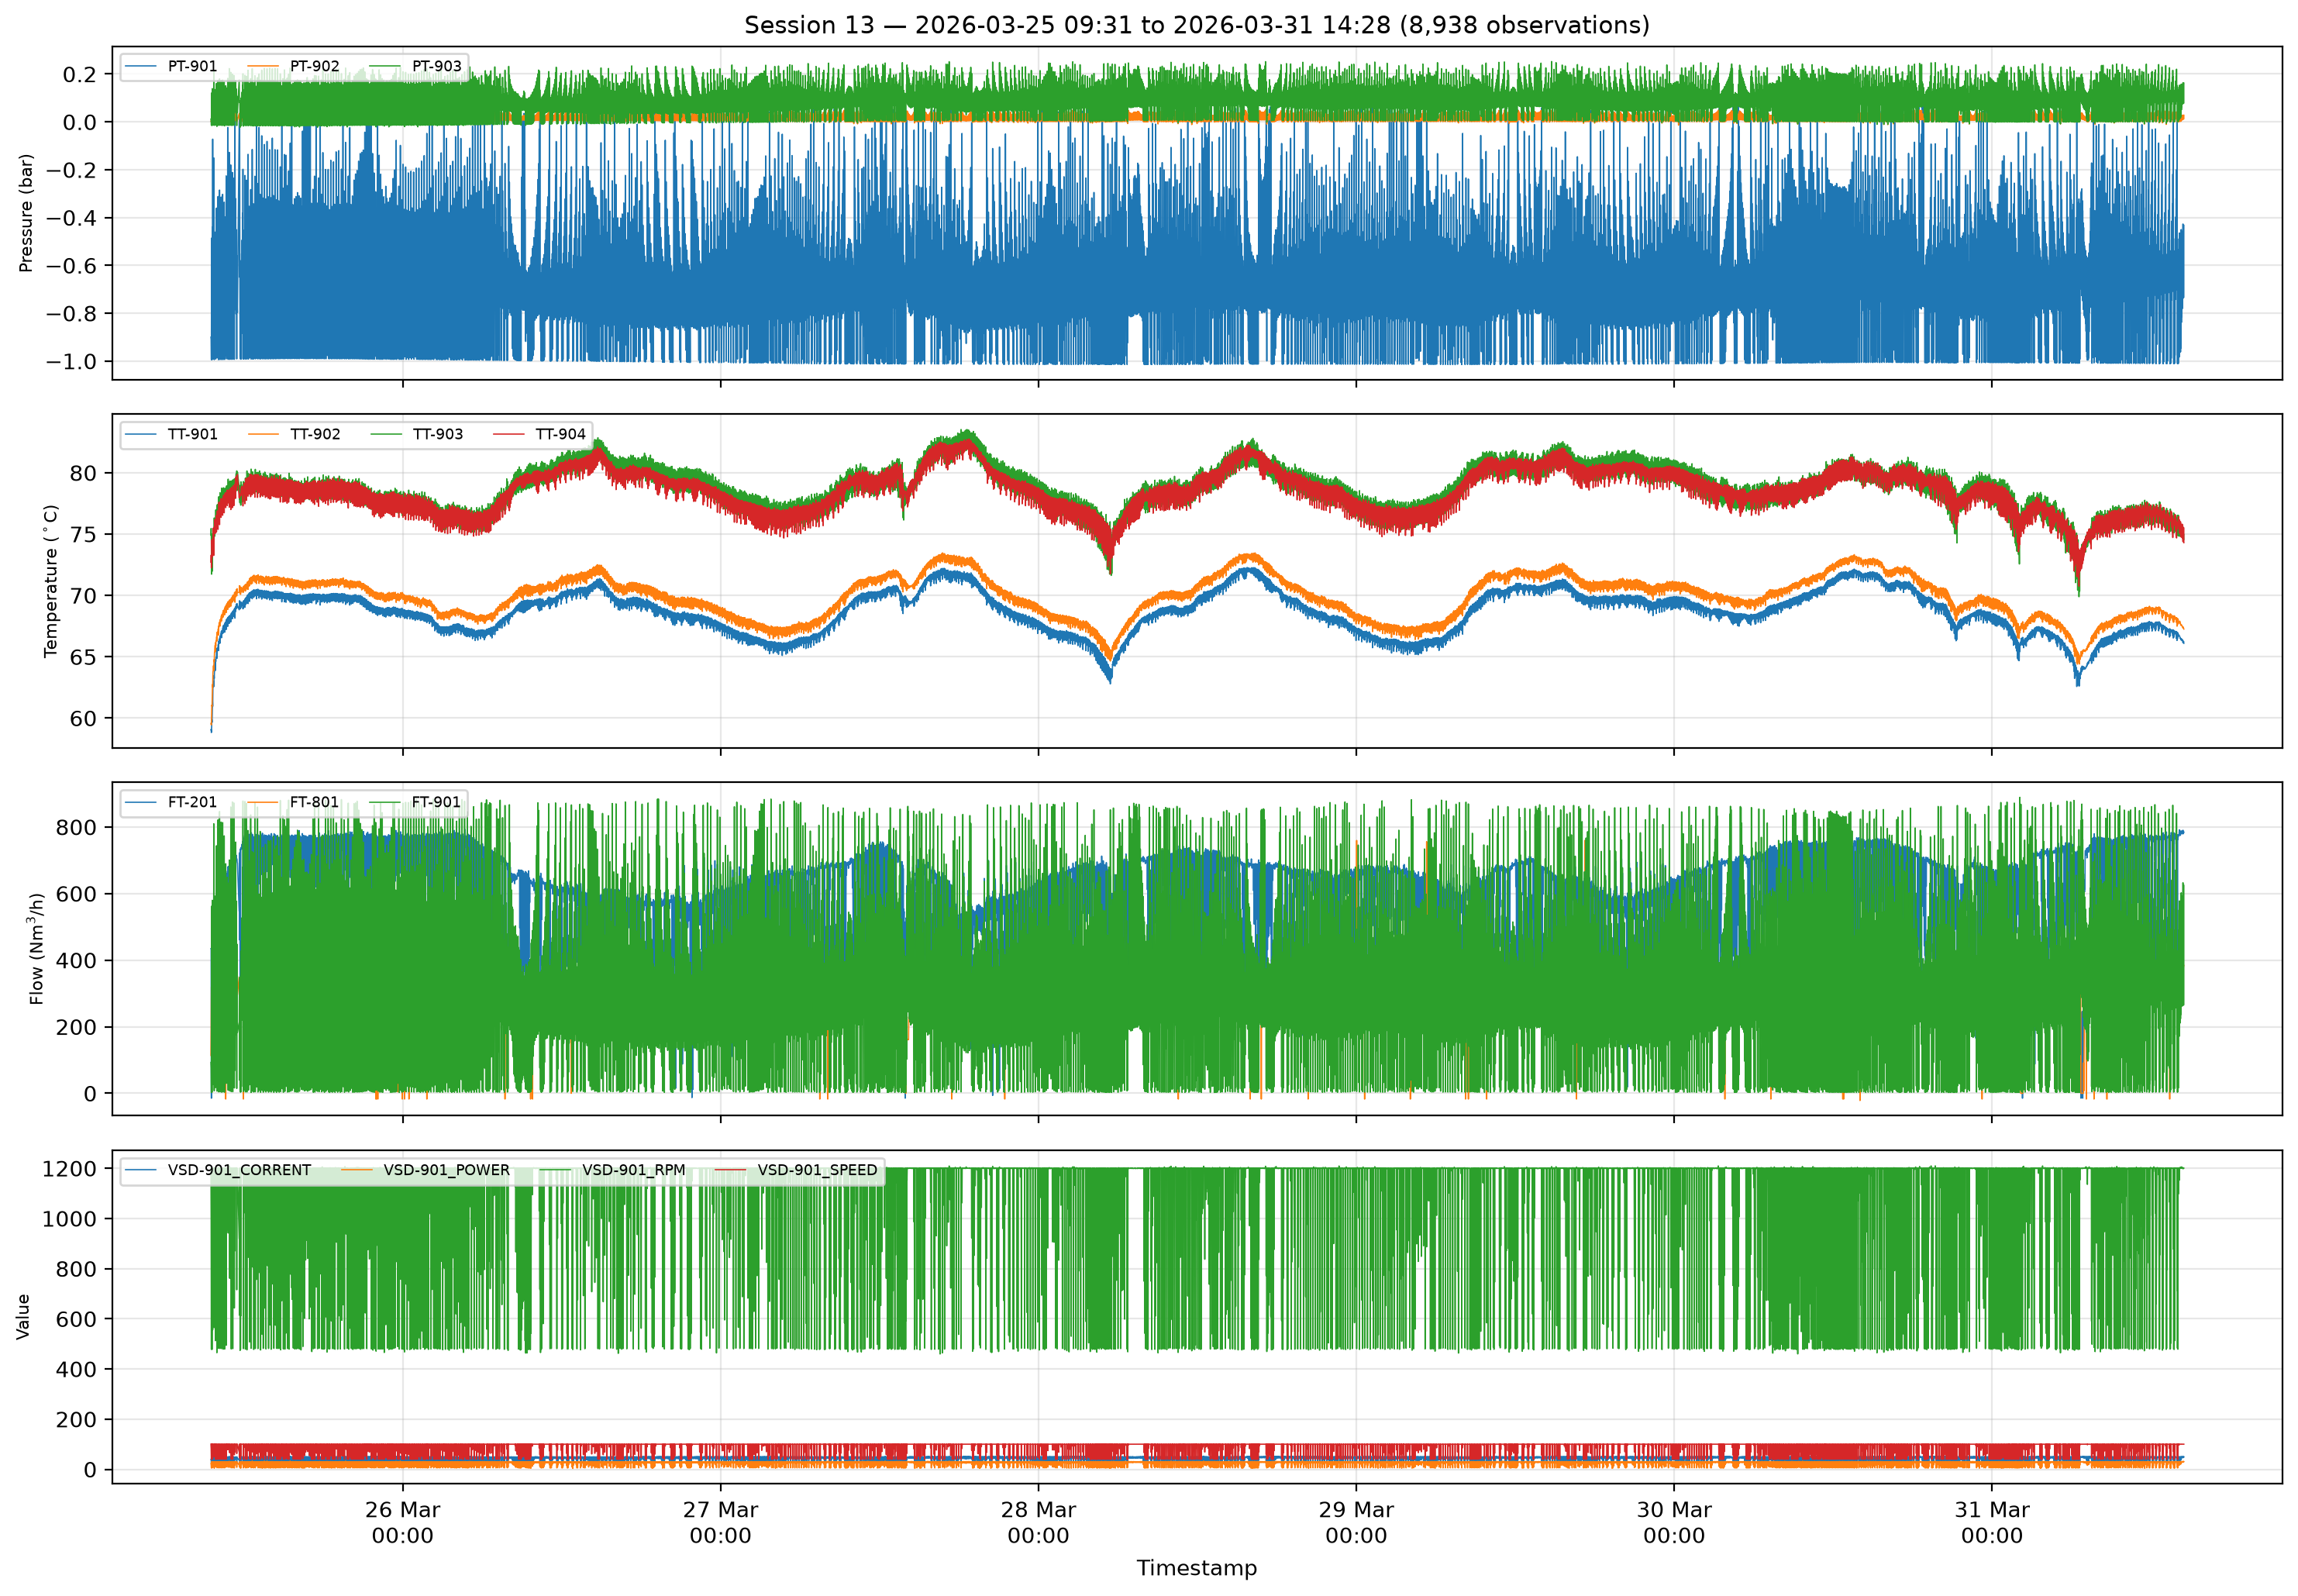
\includegraphics[width=0.95\textwidth]{imgs/eda_appendix_session_13.png}
    \caption{Session 13 (2026-03-25 09:31 to 2026-03-31 14:28, 8{,}938 observations),
    the longest session retained.}
    \label{fig:ap1_session_13}
\end{figure}

\begin{figure}[htbp]
    \centering
    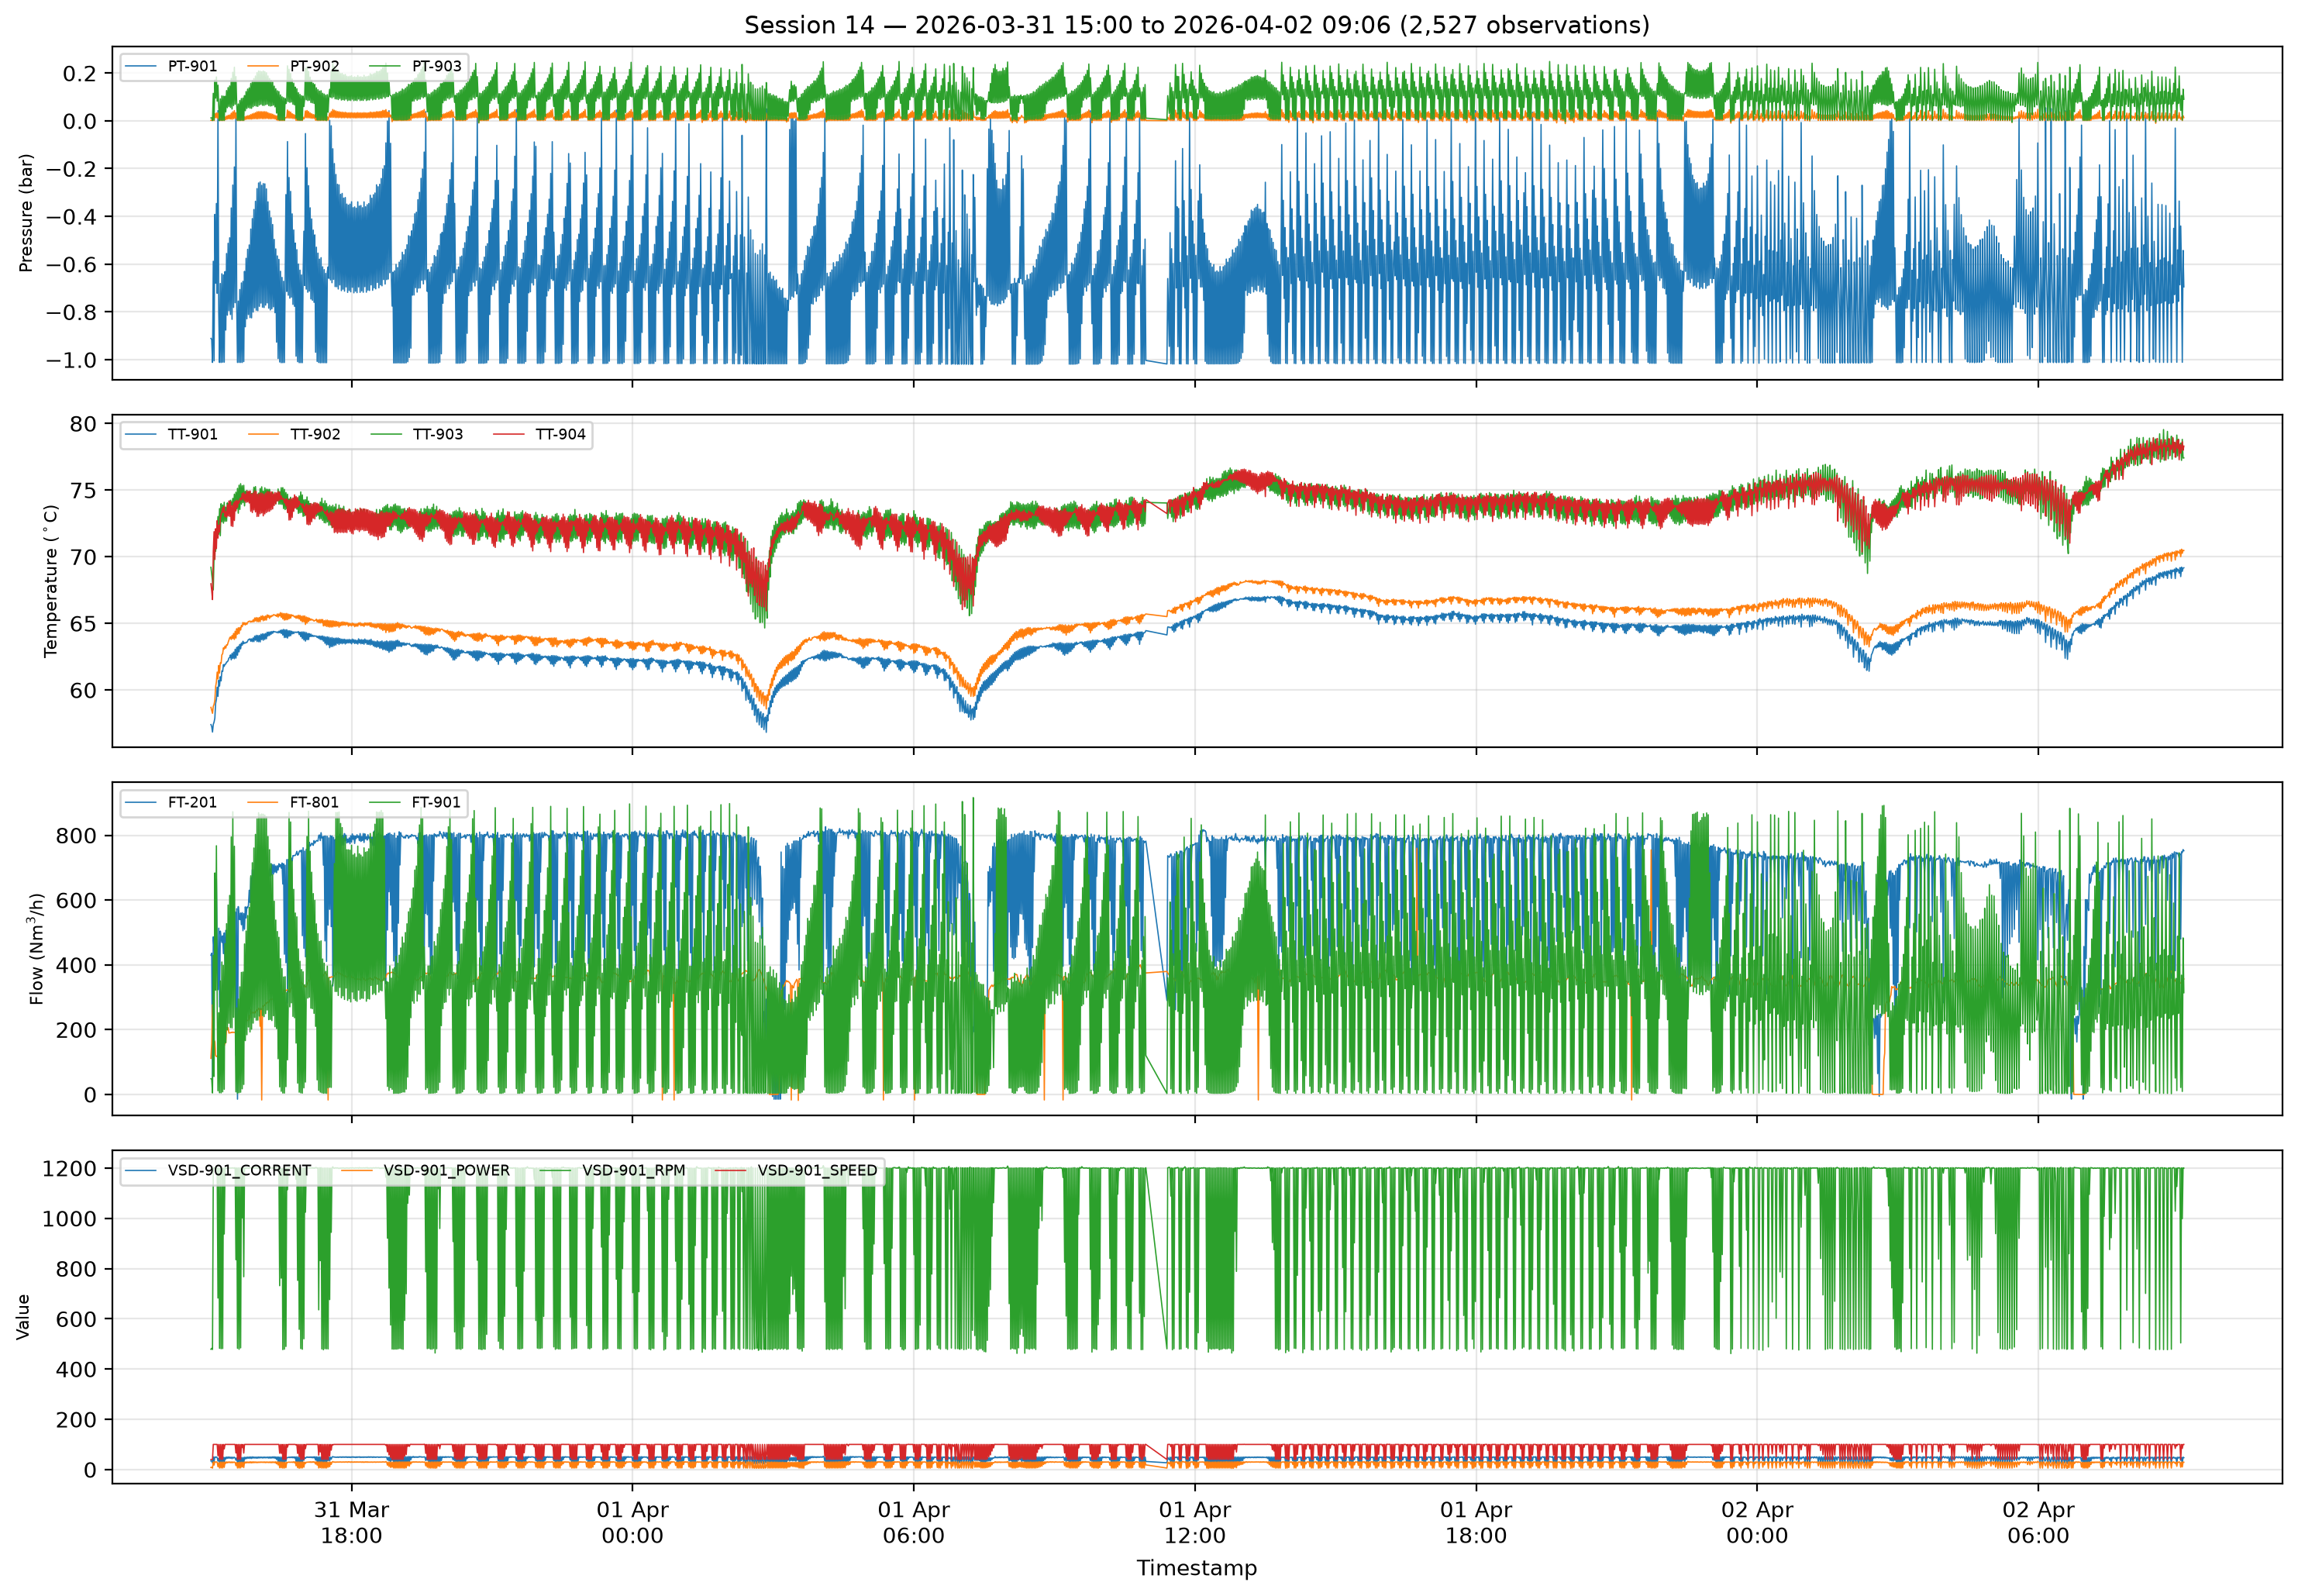
\includegraphics[width=0.95\textwidth]{imgs/eda_appendix_session_14.png}
    \caption{Session 14 (2026-03-31 15:00 to 2026-04-02 09:06, 2{,}527 observations).}
    \label{fig:ap1_session_14}
\end{figure}

\begin{figure}[htbp]
    \centering
    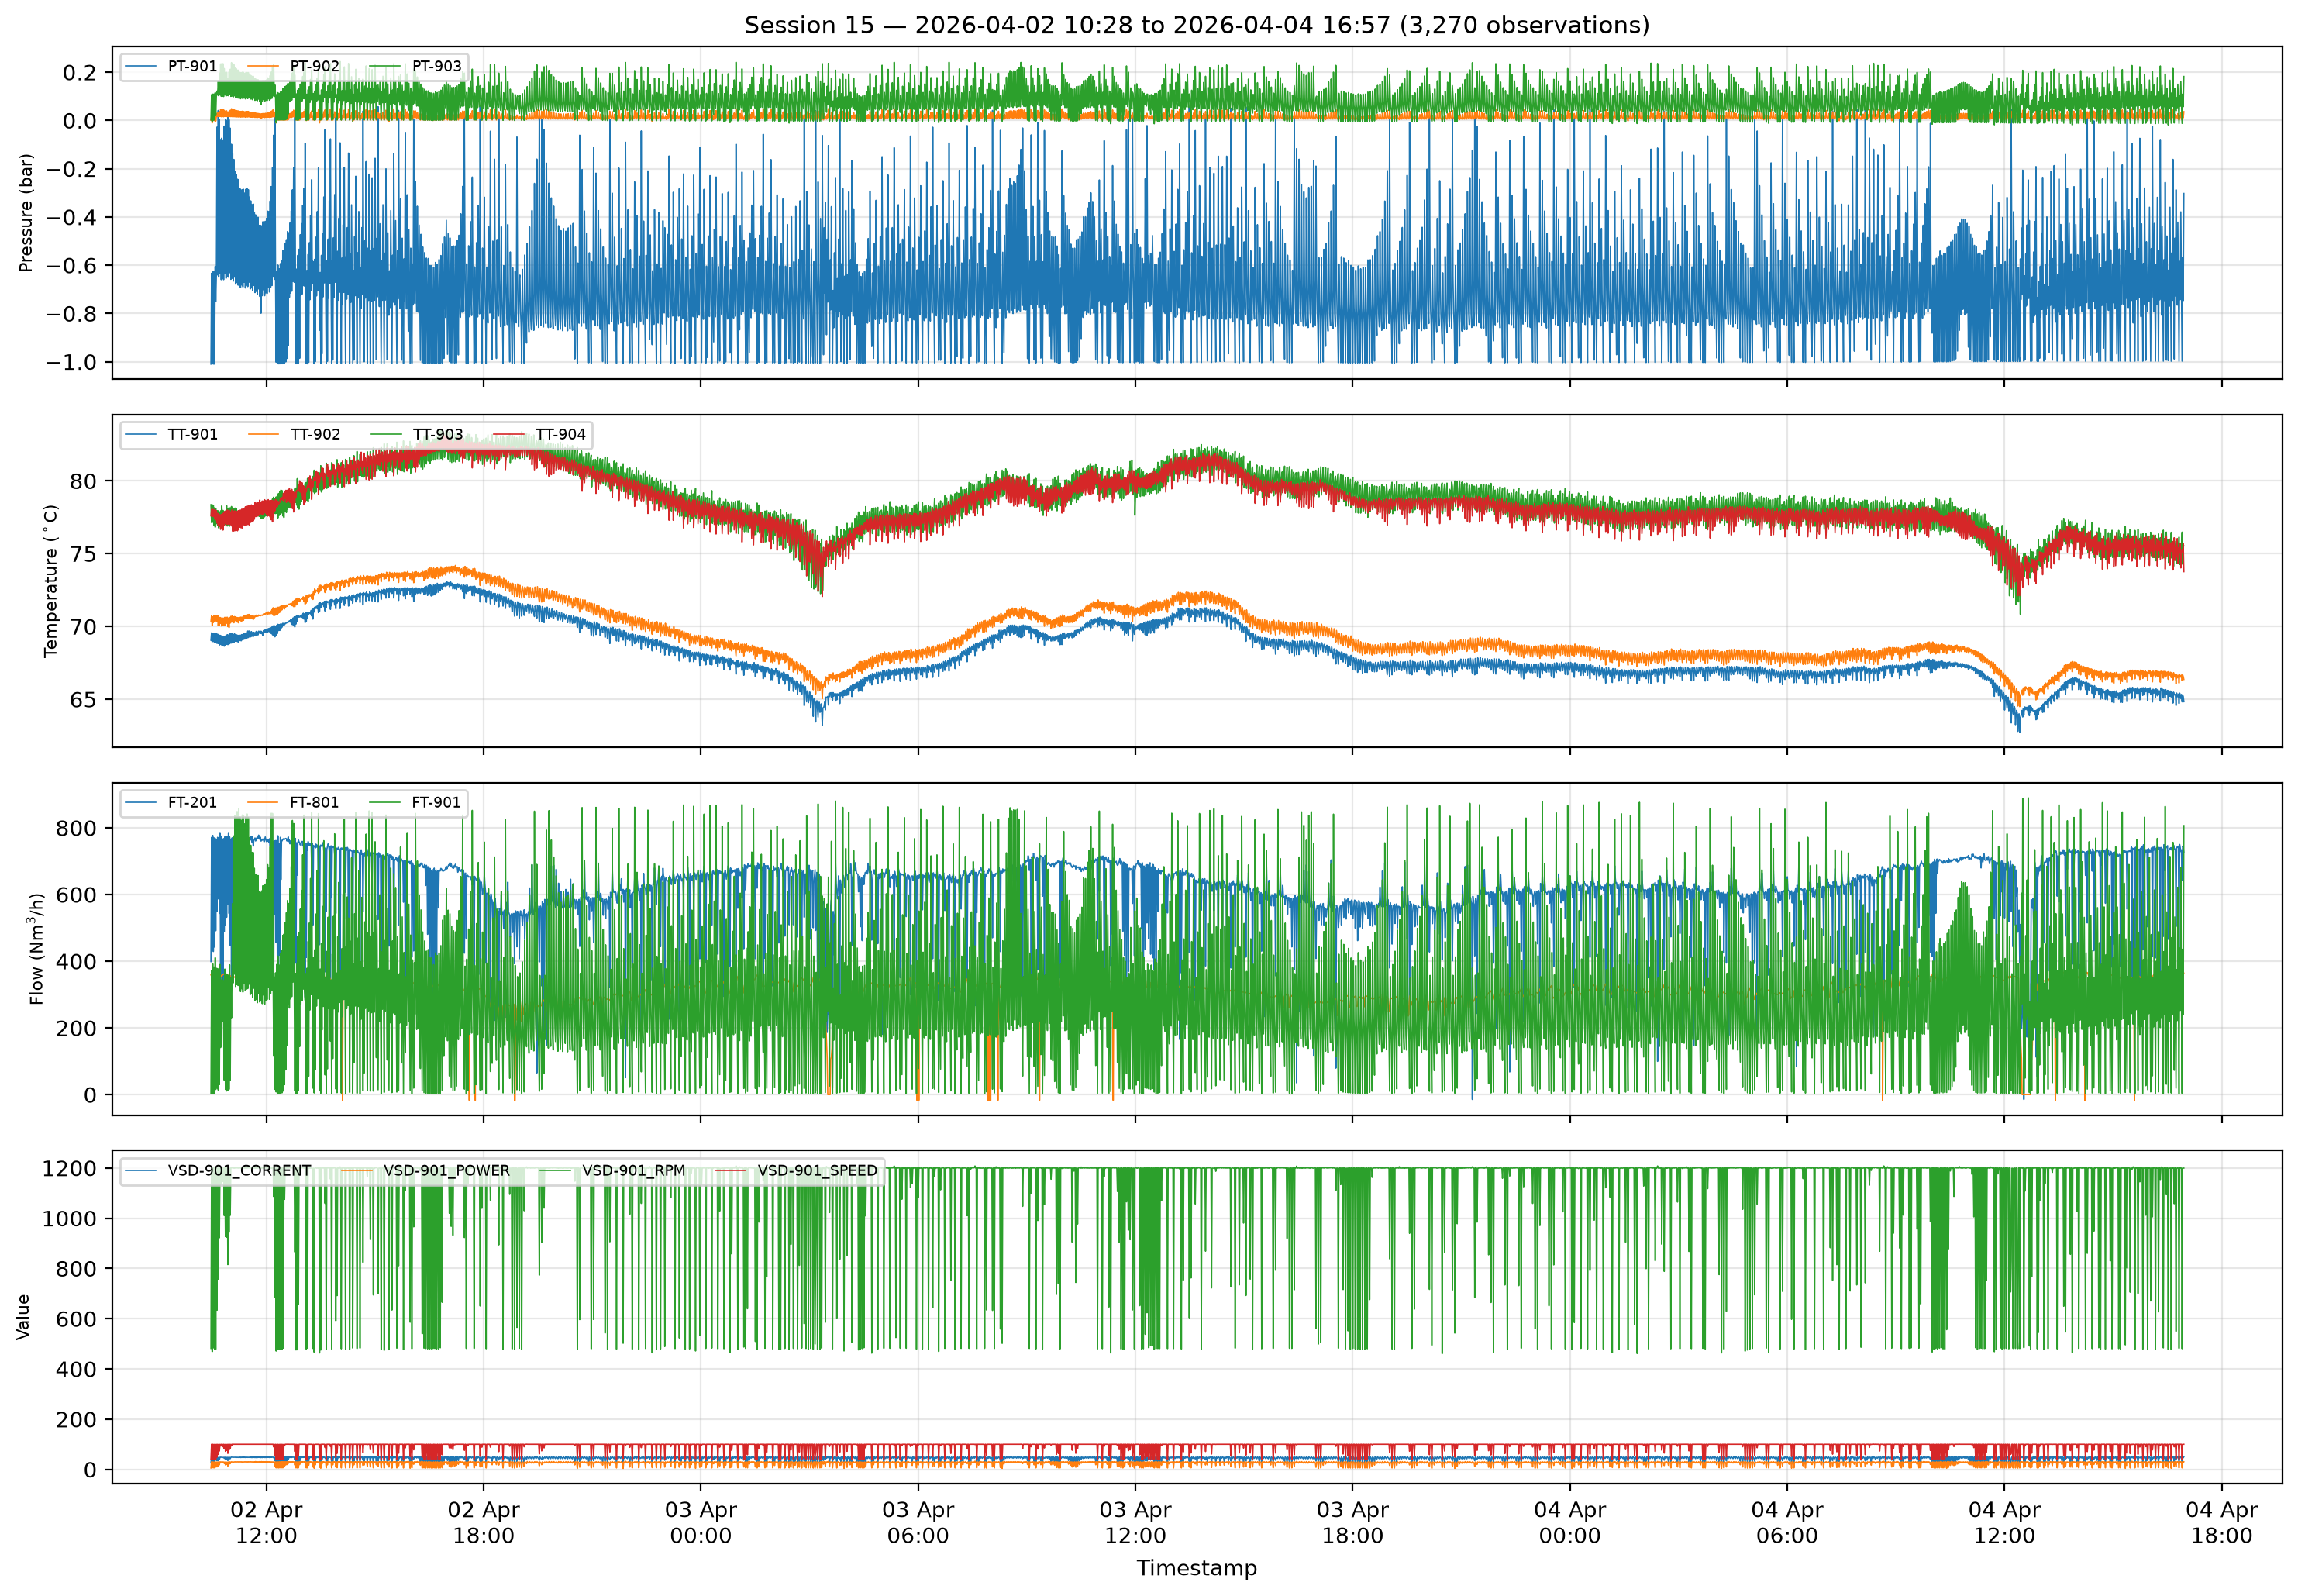
\includegraphics[width=0.95\textwidth]{imgs/eda_appendix_session_15.png}
    \caption{Session 15 (2026-04-02 10:28 to 2026-04-04 16:57, 3{,}270 observations).}
    \label{fig:ap1_session_15}
\end{figure}

\begin{figure}[htbp]
    \centering
    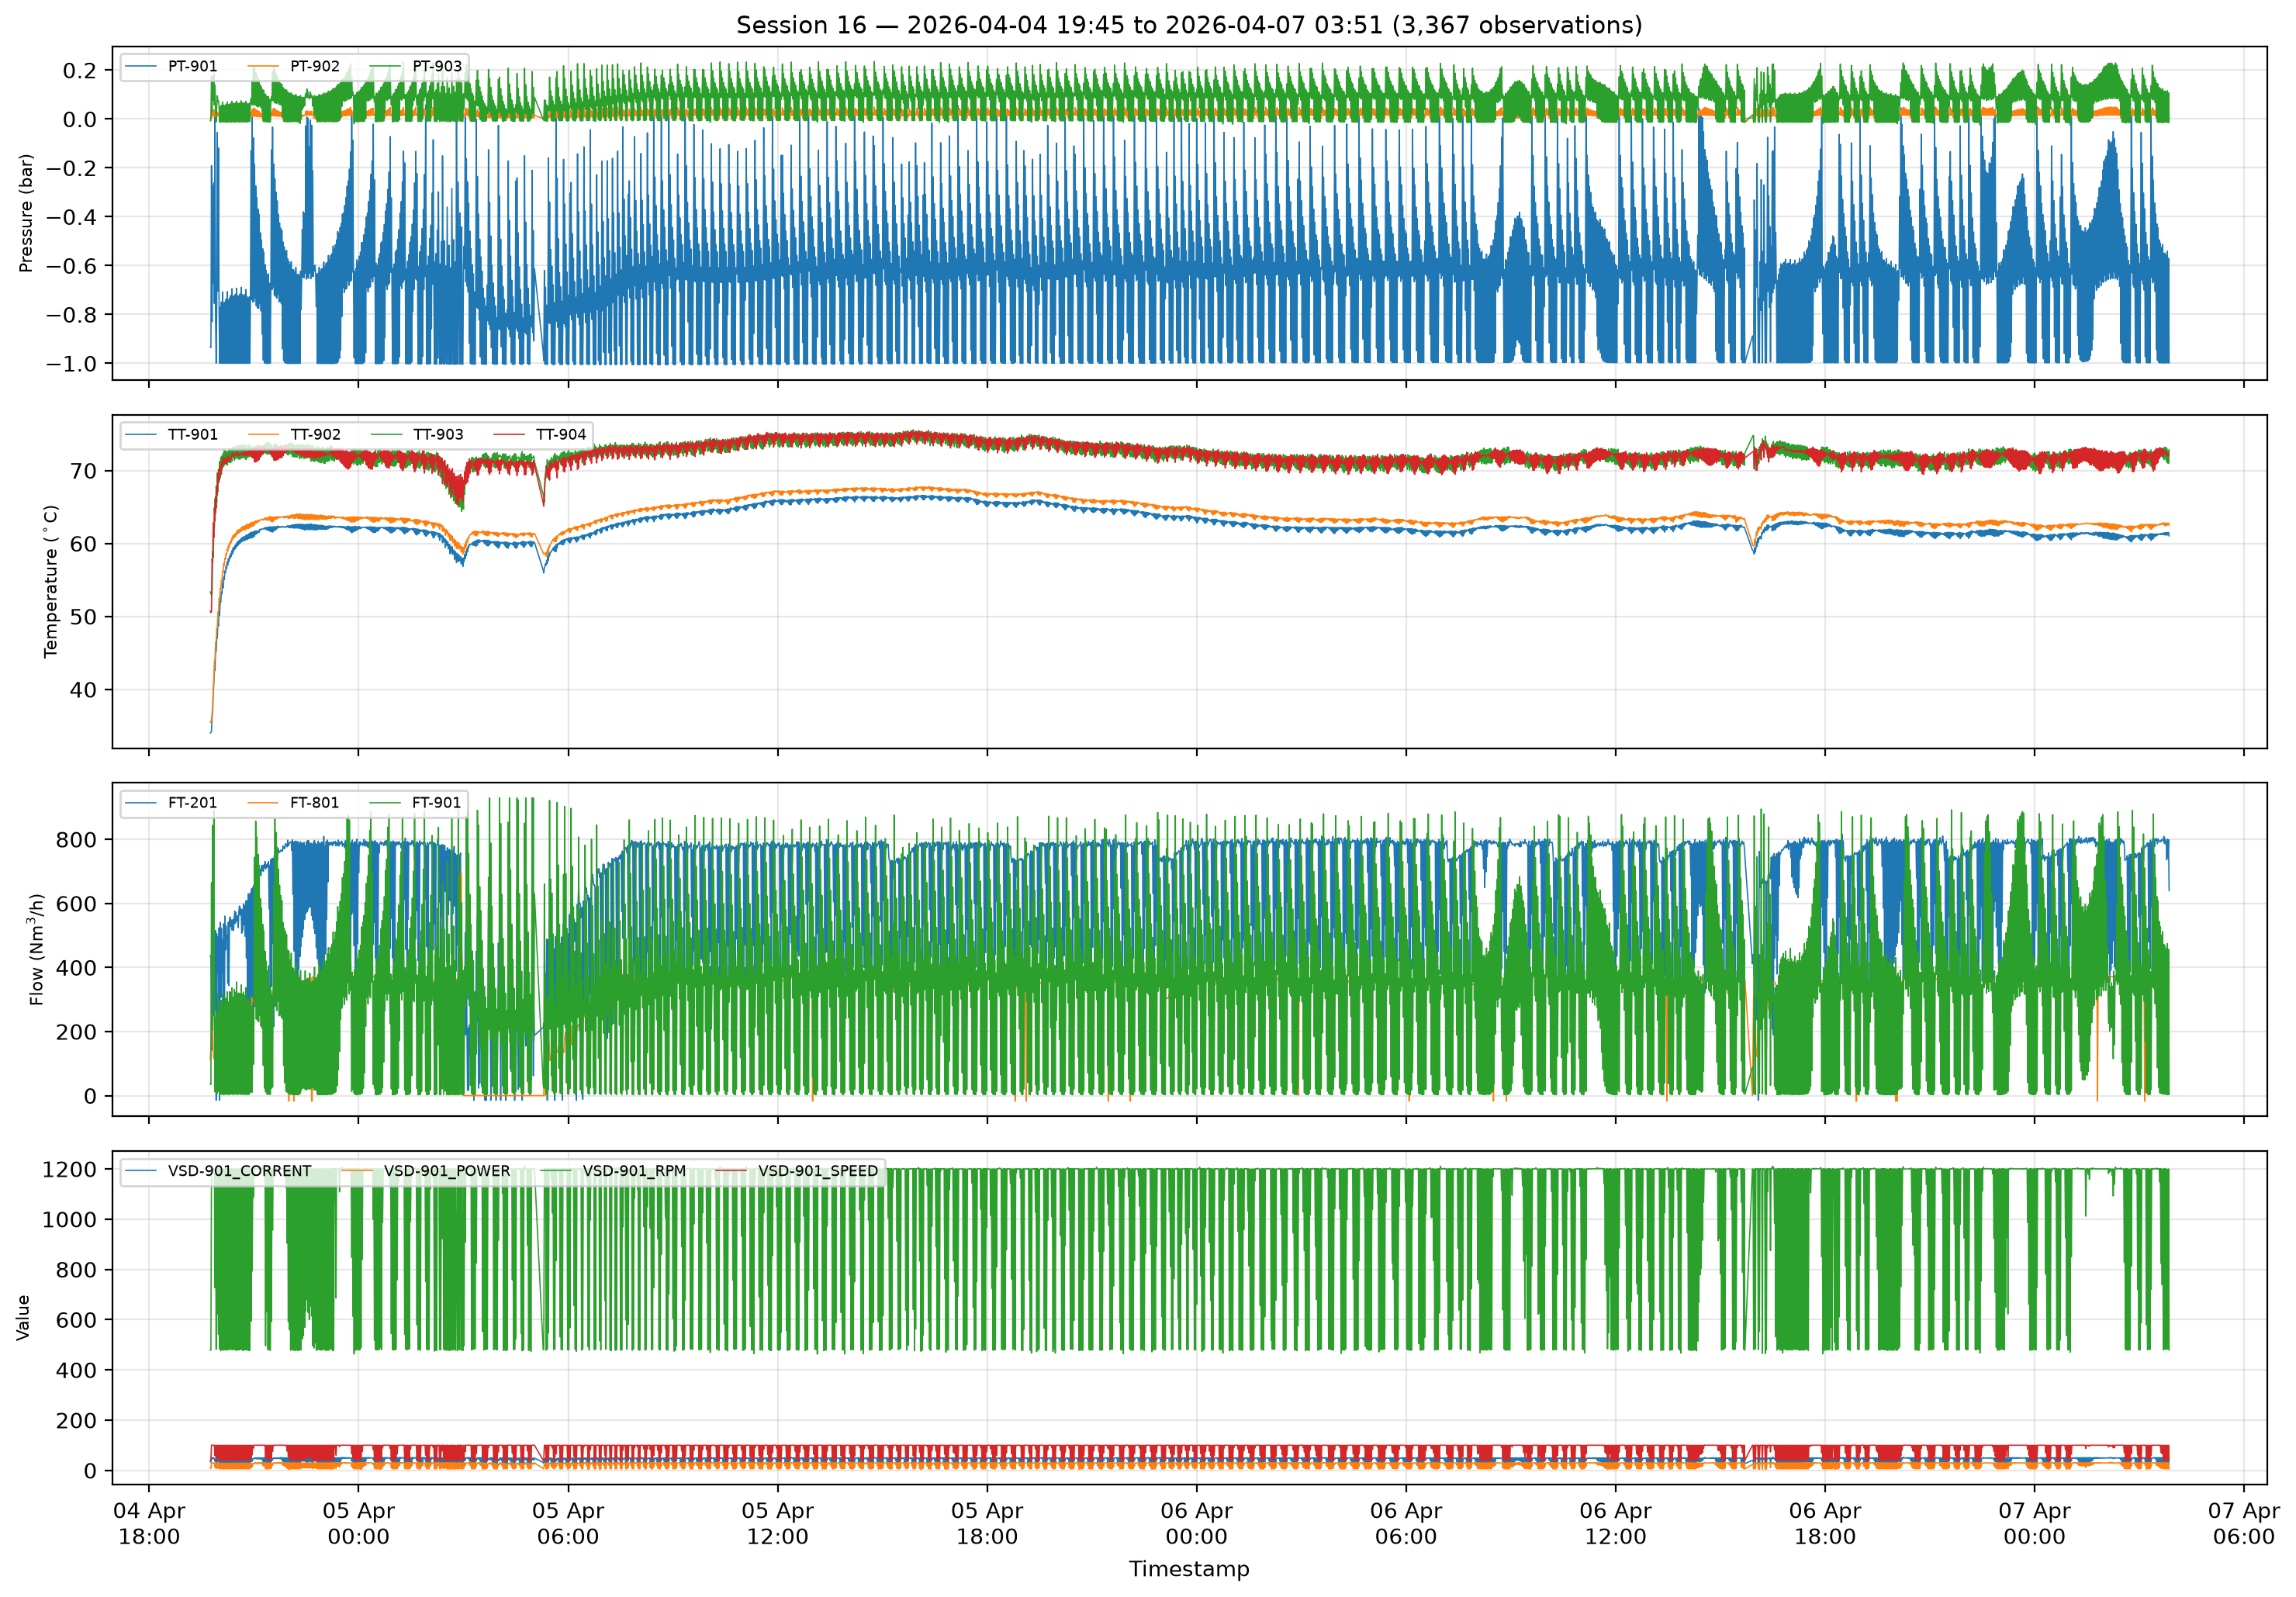
\includegraphics[width=0.95\textwidth]{imgs/eda_appendix_session_16.png}
    \caption{Session 16 (2026-04-04 19:45 to 2026-04-07 03:51, 3{,}367 observations),
    prior to fault injection.}
    \label{fig:ap1_session_16}
\end{figure}

\begin{figure}[htbp]
    \centering
    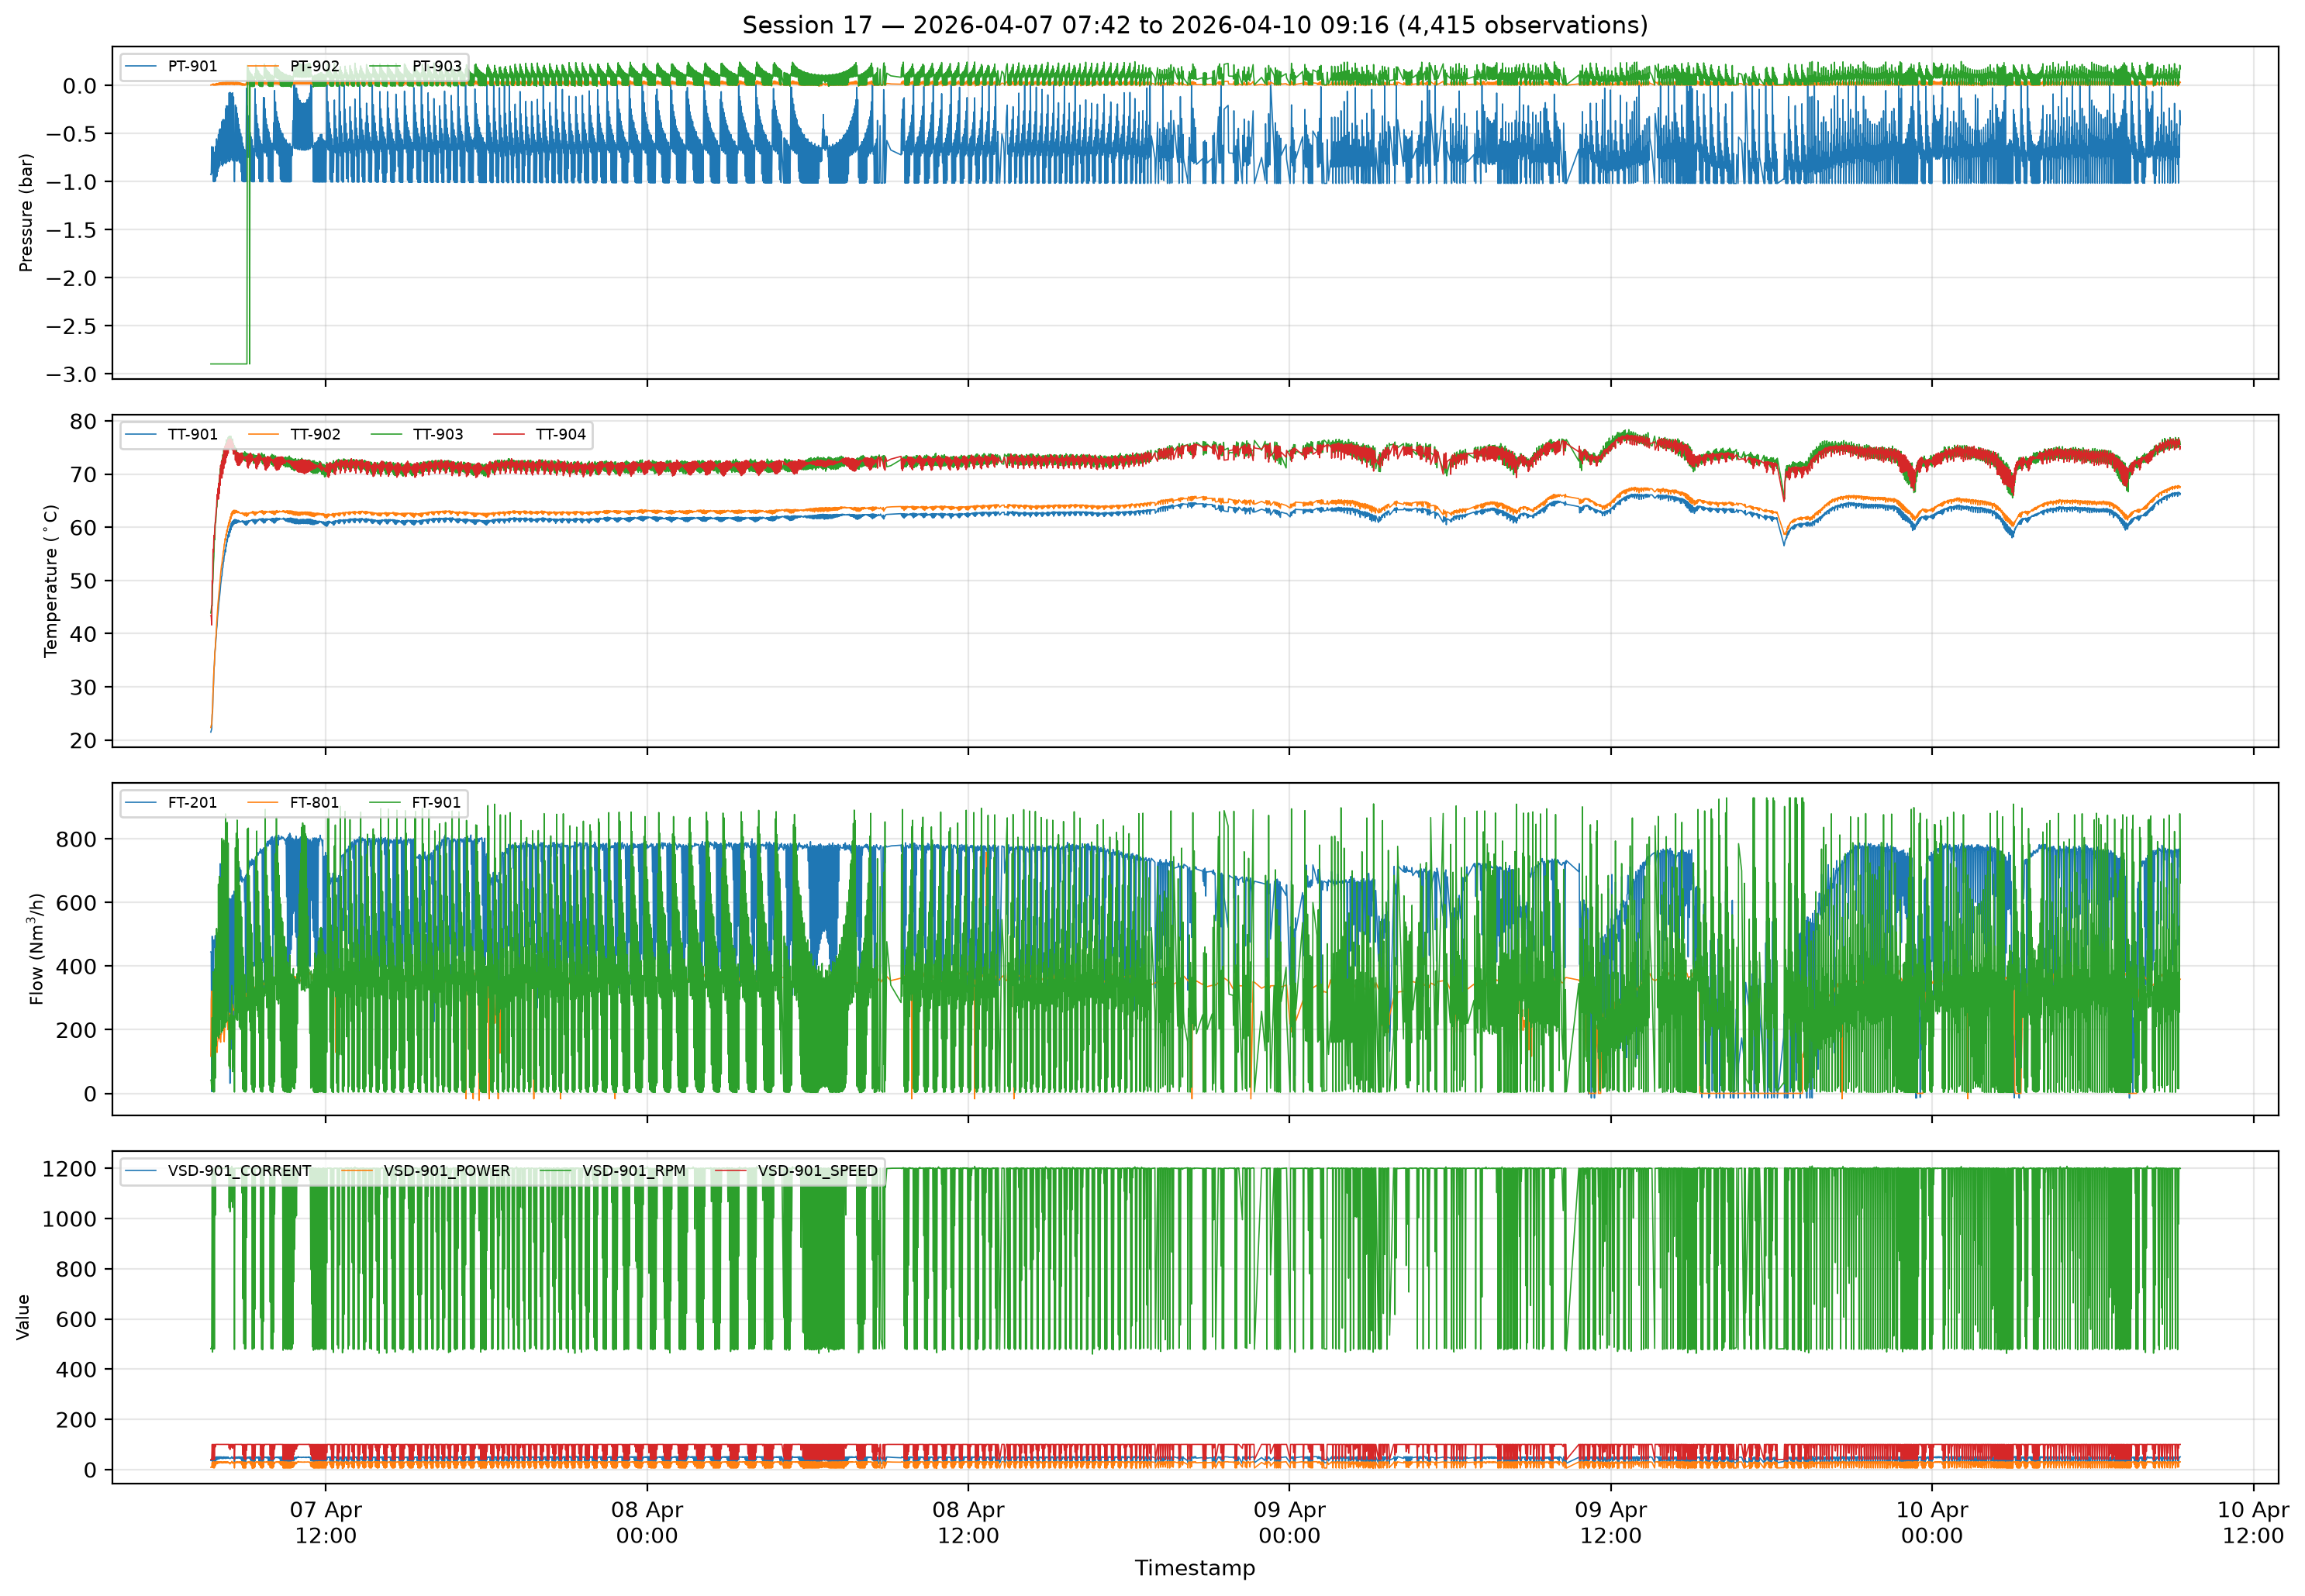
\includegraphics[width=0.95\textwidth]{imgs/eda_appendix_session_17.png}
    \caption{Session 17 (2026-04-07 07:42 to 2026-04-10 09:16, 4{,}415 observations),
    prior to fault injection. This is the session containing the frozen PT-903 episode
    discussed in Section~\ref{sec:eda}.}
    \label{fig:ap1_session_17}
\end{figure}
